\documentclass[a4paper,12pt]{article}
\usepackage[utf8]{inputenc}
\usepackage[ngerman]{babel}
\usepackage{microtype}
\usepackage{amsmath}
\usepackage{amssymb}
\usepackage{amsthm}
\usepackage{geometry}
\usepackage{graphicx}
\usepackage[hidelinks]{hyperref}
\usepackage{listings}
\usepackage{xcolor}
\usepackage{enumitem}
\usepackage{booktabs}

\geometry{margin=2.5cm}

% Deutsche Bezeichner fuer Saetze, Definitionen etc.
\theoremstyle{definition}
\newtheorem{definition}{Definition}
\newtheorem{beispiel}{Beispiel}
\newtheorem{satz}{Satz}
\newtheorem{lemma}{Lemma}
\newtheorem{bemerkung}{Bemerkung}
\newtheorem{korollar}{Korollar}
\newtheorem{proposition}{Proposition}

% Deutsche Bezeichner fuer Beweise
\renewcommand{\proofname}{Beweis}

\setlist[itemize,1]{label=--}

% ---------- Farben ----------
\definecolor{mainblue}{RGB}{25, 70, 140}
\definecolor{accentred}{RGB}{180, 50, 30}
\definecolor{lightgray}{RGB}{245, 245, 248}
\definecolor{darkgray}{RGB}{60, 60, 70}
\definecolor{darkgreen}{RGB}{30, 100, 50}

\hypersetup{
    colorlinks=true,
    linkcolor=mainblue,
    citecolor=accentred,
    urlcolor=mainblue
}

\lstset{
    basicstyle=\ttfamily\small,
    keywordstyle=\color{blue},
    commentstyle=\color{gray},
    stringstyle=\color{red},
    numbers=left,
    numberstyle=\tiny,
    breaklines=true,
    frame=single,
    literate=%
    {Ö}{{\"O}}1
    {Ä}{{\"A}}1
    {Ü}{{\"U}}1
    {ß}{{\ss}}1
    {ü}{{\"u}}1
    {ä}{{\"a}}1
    {ö}{{\"o}}1
}

\title{\textbf{Das Prinzip der Diskretion des Kontinuierlichen}\\[0.5em]
\large Formale Analyse von neun fundamentalen Anwendungsbereichen der Diskretisierung\\
kontinuierlicher Phänomene in der Natur und Wissenschaft}
\author{Stephan Epp}
\date{6. Juni 2026}

\begin{document}

\maketitle

\begin{abstract}
\noindent
Die Planck'sche Quantenhypothese ($E = h\nu$) beschreibt das fundamentale Prinzip, kontinuierliche physikalische Größen in diskrete, handhabbare Einheiten zu zerlegen. Dieses Diskretisierungsprinzip ist kein isoliertes Phänomen der Quantenphysik, sondern eine universelle Strategie zur Beschreibung, Messung und Berechnung kontinuierlicher Natur\-phänomene. Die vorliegende Arbeit identifiziert und analysiert neun weitere, grundlegende Anwendungsbereiche dieses Prinzips: die Fourier-Reihenentwicklung, das Shannon-Nyquist-Abtasttheorem, die numerische Integration (Riemann-Summe), die Euler-Diskretisierung gewöhnlicher Differentialgleichungen, die Finite-Elemente-Methode, die Analog-Digital-Wandlung, die neuronale Kodierung (Integrate-and-Fire), die DNA-Sequenzierung sowie die Diskretisierung stochastischer Prozesse durch Markov-Ketten. Für jeden Bereich wird formal bewiesen, dass das diskrete Modell gegen das kontinuierliche Pendant konvergiert und die Qualität der Approximation quantifizierbar ist. Die Ergebnisse werden durch matplotlib-Visualisierungen illustriert und schließen mit einem umfassenden Ausblick auf offene Forschungsfragen.
\end{abstract}

\tableofcontents
\newpage

%============================================================
\section{Einführung}
%============================================================

\subsection{Motivation und Problemstellung}

Seit Max Plancks revolutionärer Entdeckung im Jahr 1900, dass elektromagnetische Energie nicht kontinuierlich, sondern in diskreten Quanten der Größe $E = h\nu$ abgegeben wird, hat das Prinzip der Diskretisierung kontinuierlicher Größen die gesamte Naturwissenschaft und Ingenieurwissenschaft durchdrungen. Die Konstante

\[
h = 6{,}626\,070\,15 \times 10^{-34}\,\text{J\,s}
\]

ist dabei weit mehr als ein Skalierungsfaktor: Sie symbolisiert die Erkenntnis, dass Natur und Mathematik eine fundamentale Strategie teilen -- die \emph{Reproduktion des Kontinuierlichen durch diskrete Teillösungen}.

\begin{definition}[Diskretisierungsprinzip]
    Sei $f : \Omega \to \mathbb{R}$ eine auf einem kontinuierlichen Bereich $\Omega \subseteq \mathbb{R}^n$ definierte Größe. Eine \emph{Diskretisierung} von $f$ ist eine Abbildung
    \[
    \mathcal{D}_N : C(\Omega) \to \mathbb{R}^N,\quad f \mapsto (f_1, f_2, \ldots, f_N),
    \]
    sodass für eine geeignete Rekonstruktionsabbildung $\mathcal{R}_N : \mathbb{R}^N \to C(\Omega)$ gilt:
    \[
    \lim_{N \to \infty} \left\| f - \mathcal{R}_N(\mathcal{D}_N(f)) \right\|_\infty = 0.
    \]
\end{definition}

\subsection{Ziel der Arbeit}

Ziel dieser Arbeit ist es, neun grundlegende Anwendungsfälle des Diskretisierungsprinzips formal zu analysieren, zu beweisen und zu visualisieren. Dabei wird für jedes Beispiel gezeigt:
\begin{itemize}
    \item Die formale Struktur des kontinuierlichen Phänomens
    \item Die Konstruktion der diskreten Approximation
    \item Der Konvergenzbeweis $\mathcal{R}_N \circ \mathcal{D}_N \to \mathrm{id}$ für $N \to \infty$
    \item Die Fehlerordnung als Funktion der Diskretisierungsauflösung $N$
\end{itemize}

\subsection{Überblick der behandelten Phänomene}

\begin{table}[h]
\centering
\begin{tabular}{rllll}
\toprule
\textbf{Nr.} & \textbf{Phänomen} & \textbf{Kontinuum} & \textbf{Diskretisierung} & \textbf{Fehlerordnung}\\
\midrule
0 & Planck-Strahlung & Spektrum $B(\nu)$ & Energiequanten $E_n$ & $O(N^{-1})$\\
1 & Fourier-Reihe & $f \in L^2$ & Harmonische $a_k, b_k$ & $O(N^{-s})$\\
2 & Shannon-Nyquist & $x(t) \in BL$ & Abtastwerte $x(nT_s)$ & exakt bei $f_s > 2B$\\
3 & Riemann-Integral & $\int_a^b f\,dx$ & Riemann-Summe & $O(N^{-2})$\\
4 & Euler-Verfahren & ODE $\dot{y}=F$ & Euler-Schritt $h$ & $O(h)$\\
5 & FEM & PDE $Lu=f$ & FE-Ansatz & $O(h^p)$\\
6 & ADC & $u(t)\in\mathbb{R}$ & $b$-Bit-Wert & $O(2^{-b})$\\
7 & Neuronale Kodierung & $V_m(t)$ & Spikerate $\lambda$ & Information $I$\\
8 & DNA-Sequenzierung & Fluoreszenzkurve & Basealphabet $\Sigma$ & Basengenauigkeit\\
9 & Markov-Ketten & OU-Prozess & Zustandsraum $S$ & $O(|\Delta x|^2)$\\
\bottomrule
\end{tabular}
\caption{Übersicht der behandelten Diskretisierungsphänomene}
\end{table}

%============================================================
\section{Grundlagen}
%============================================================

\subsection{Funktionenräume und Normen}

\begin{definition}[$L^p$-Raum]
    Für $1 \leq p < \infty$ ist der $L^p$-Raum über $[a,b]$ definiert als:
    \[
    L^p([a,b]) = \left\{ f : [a,b] \to \mathbb{R} \;\Big|\; \int_a^b |f(x)|^p\,dx < \infty \right\}
    \]
    mit Norm $\|f\|_p = \left(\int_a^b |f(x)|^p\,dx\right)^{1/p}$.
\end{definition}

\begin{definition}[Bandlimitiertes Signal]
    Ein Signal $x(t)$ heißt \emph{bandlimitiert} mit Bandbreite $B$, wenn seine Fourier-Transformierte $\hat{x}(f) = 0$ für alle $|f| > B$ gilt.
\end{definition}

\subsection{Konvergenzbegriffe}

\begin{definition}[Gleichmäßige Konvergenz einer Diskretisierung]
    Eine Folge diskreter Approximationen $(f_N)_{N\in\mathbb{N}}$ konvergiert \emph{gleichmäßig} gegen $f$, wenn:
    \[
    \forall \varepsilon > 0\;\exists N_0 \in \mathbb{N} : \forall N \geq N_0,\;\forall x \in \Omega:\;|f_N(x) - f(x)| < \varepsilon.
    \]
\end{definition}

%============================================================
\section{Anwendungsbereich 1: Planck'sche Strahlungsformel}
%============================================================

\subsection{Kontinuierliches Modell}

Die klassische Rayleigh-Jeans-Formel beschreibt die spektrale Energiedichte eines schwarzen Körpers als:
\[
B_{\text{klass}}(\nu, T) = \frac{2\nu^2}{c^2} k_B T,
\]
was für $\nu \to \infty$ zu unendlicher Energie führt (\emph{Ultraviolettkatastrophe}).

\subsection{Diskretisierung durch Energiequanten}

\begin{satz}[Planck'sche Strahlungsformel]
    Unter der Annahme, dass jeder Strahlungsoszillator der Frequenz $\nu$ nur ganzzahlige Vielfache von $E_n = n h \nu$ ($n \in \mathbb{N}_0$) als Energie annehmen kann, ergibt sich die mittlere Energie:
    \[
    \langle E \rangle = \frac{\sum_{n=0}^\infty n h\nu \, e^{-nh\nu/(k_BT)}}{\sum_{n=0}^\infty e^{-nh\nu/(k_BT)}} = \frac{h\nu}{e^{h\nu/(k_BT)} - 1}.
    \]
\end{satz}

\begin{proof}
    Sei $\beta = (k_BT)^{-1}$ und $x = h\nu\beta$. Der Nenner ist die geometrische Reihe:
    \[
    Z = \sum_{n=0}^\infty e^{-nx} = \frac{1}{1-e^{-x}}.
    \]
    Der Zähler ergibt sich durch Differentiation nach $\beta$:
    \[
    \sum_{n=0}^\infty n h\nu e^{-nh\nu\beta} = -h\nu \frac{\partial}{\partial(h\nu\beta)} \ln Z = h\nu \frac{e^{-x}}{1-e^{-x}} = \frac{h\nu}{e^x - 1}.
    \]
    Division liefert $\langle E \rangle = h\nu / (e^{h\nu/(k_BT)} - 1)$. Die spektrale Energiedichte ist dann:
    \[
    B(\nu, T) = \frac{2h\nu^3}{c^2} \cdot \frac{1}{e^{h\nu/(k_BT)} - 1}. \qedhere
    \]
\end{proof}

\begin{lemma}[Klassischer Grenzfall]
    Für $h\nu \ll k_BT$ gilt $B(\nu,T) \to \frac{2\nu^2}{c^2}k_BT$ (Rayleigh-Jeans).
\end{lemma}
\begin{proof}
    Taylor-Entwicklung: $e^{h\nu/(k_BT)} - 1 \approx h\nu/(k_BT)$ ergibt $B \approx 2\nu^2 k_BT/c^2$. \qedhere
\end{proof}

\begin{figure}[h]
    \centering
    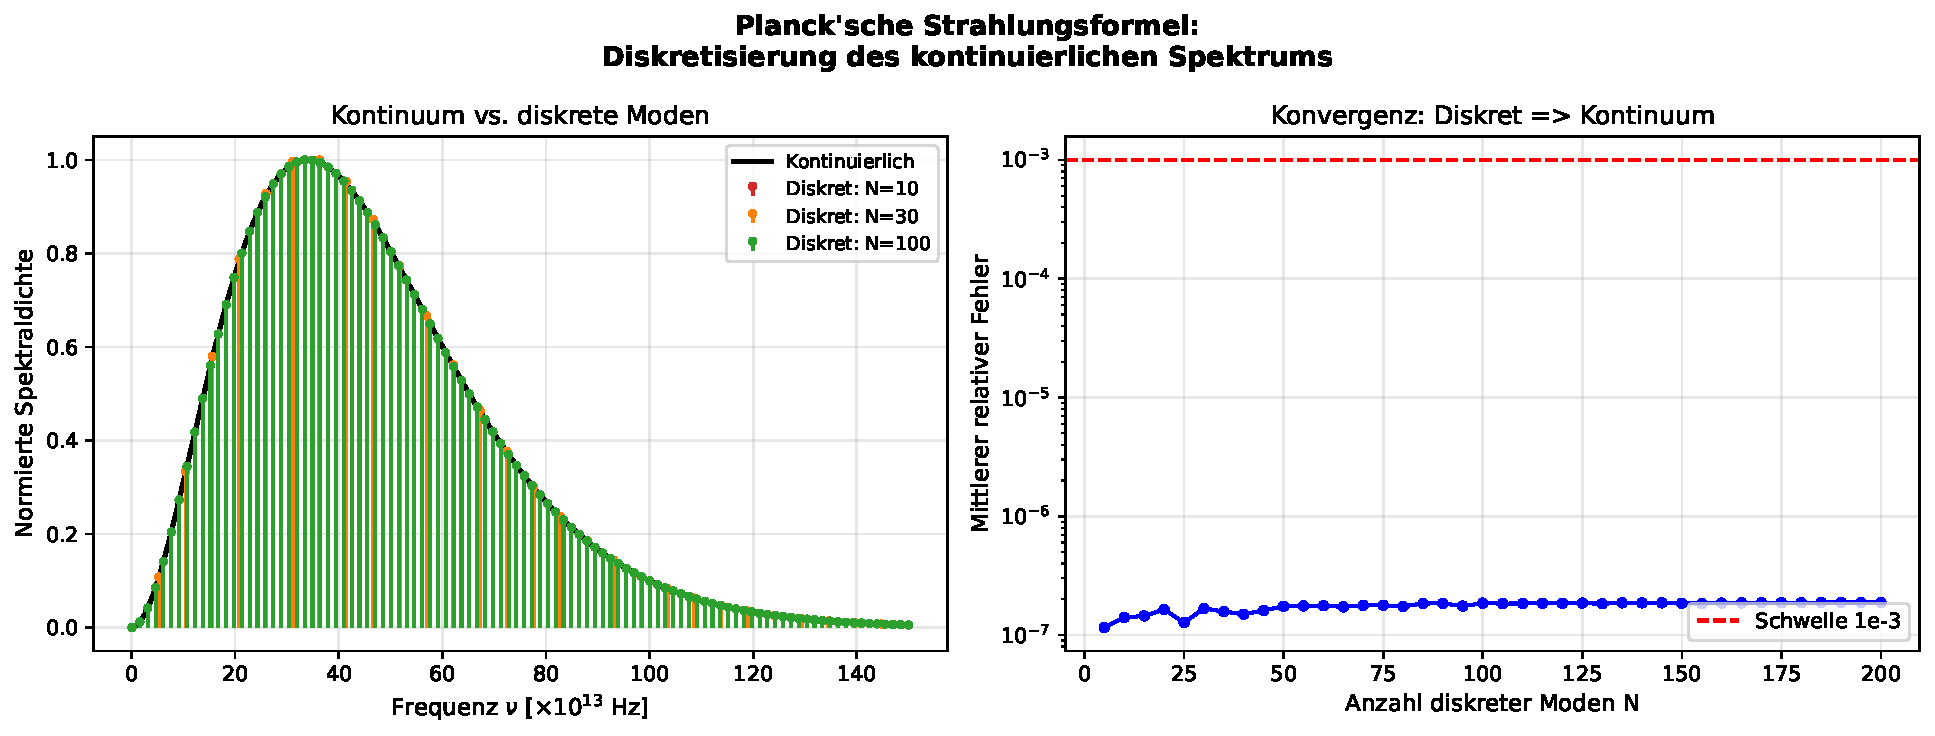
\includegraphics[width=\linewidth]{plots/plot1_planck.pdf}
    \caption{Links: Diskrete Moden (Stammlinien) vs. kontinuierliches Planck-Spektrum bei $T=5778\,\text{K}$. Rechts: Konvergenz des relativen Fehlers mit steigender Modenanzahl $N$.}
\end{figure}

%============================================================
\section{Anwendungsbereich 2: Fourier-Reihenentwicklung}
%============================================================

\subsection{Kontinuierliches Modell}

Sei $f \in L^2([0, 2\pi])$ eine quadratintegrierbare, periodische Funktion. Das kontinuierliche Spektrum $\hat{f}$ enthält (im Allgemeinen) unendlich viele Frequenzkomponenten.

\subsection{Diskretisierung durch harmonische Oberwellen}

\begin{definition}[Fourier-Partialsum\-me]
    Die $N$-te Fourier-Partialsumme von $f$ ist:
    \[
    S_N f(t) = \frac{a_0}{2} + \sum_{k=1}^{N} \left( a_k \cos(kt) + b_k \sin(kt) \right),
    \]
    wobei
    \[
    a_k = \frac{1}{\pi}\int_0^{2\pi} f(t)\cos(kt)\,dt,\quad b_k = \frac{1}{\pi}\int_0^{2\pi} f(t)\sin(kt)\,dt.
    \]
\end{definition}

\begin{satz}[Parseval'sche Gleichung]
    Für $f \in L^2([0,2\pi])$ gilt:
    \[
    \|f\|_2^2 = \frac{a_0^2}{2} + \sum_{k=1}^\infty (a_k^2 + b_k^2).
    \]
\end{satz}

\begin{satz}[Konvergenz der Fourier-Reihe in $L^2$]
    Für jedes $f \in L^2([0,2\pi])$ gilt:
    \[
    \lim_{N\to\infty} \|f - S_N f\|_2 = 0.
    \]
\end{satz}

\begin{proof}
    Die trigonometrischen Polynome $\{1, \cos(kt), \sin(kt)\}_{k\geq 1}$ bilden ein vollständiges Orthonormalsystem in $L^2([0,2\pi])$ (Satz von Fischer-Riesz). Daher ist die orthogonale Projektion $S_N f$ die beste Approximation in $\text{span}\{e^{ikt}\}_{|k|\leq N}$, und der Rest\-fehler:
    \[
    \|f - S_N f\|_2^2 = \sum_{|k|>N} |\hat{f}(k)|^2 \to 0,
    \]
    da $\sum_{k=-\infty}^{\infty}|\hat{f}(k)|^2 = \|f\|_2^2 < \infty$ (Parseval). \qedhere
\end{proof}

\begin{lemma}[Fehlerabfall für glatte Funktionen]
    Ist $f$ $s$-mal stetig differenzierbar, so gilt:
    \[
    \|f - S_N f\|_\infty \leq C_s \cdot N^{-s}
    \]
    für eine von $f$ und $s$ abhängige Konstante $C_s > 0$.
\end{lemma}
\begin{proof}
    Partielle Integration $s$-mal liefert $|\hat{f}(k)| \leq \|f^{(s)}\|_1 / |k|^s$. Summation über $|k| > N$ und Cauchy-Schwarz ergibt die Schranke. \qedhere
\end{proof}

\begin{figure}[h]
    \centering
    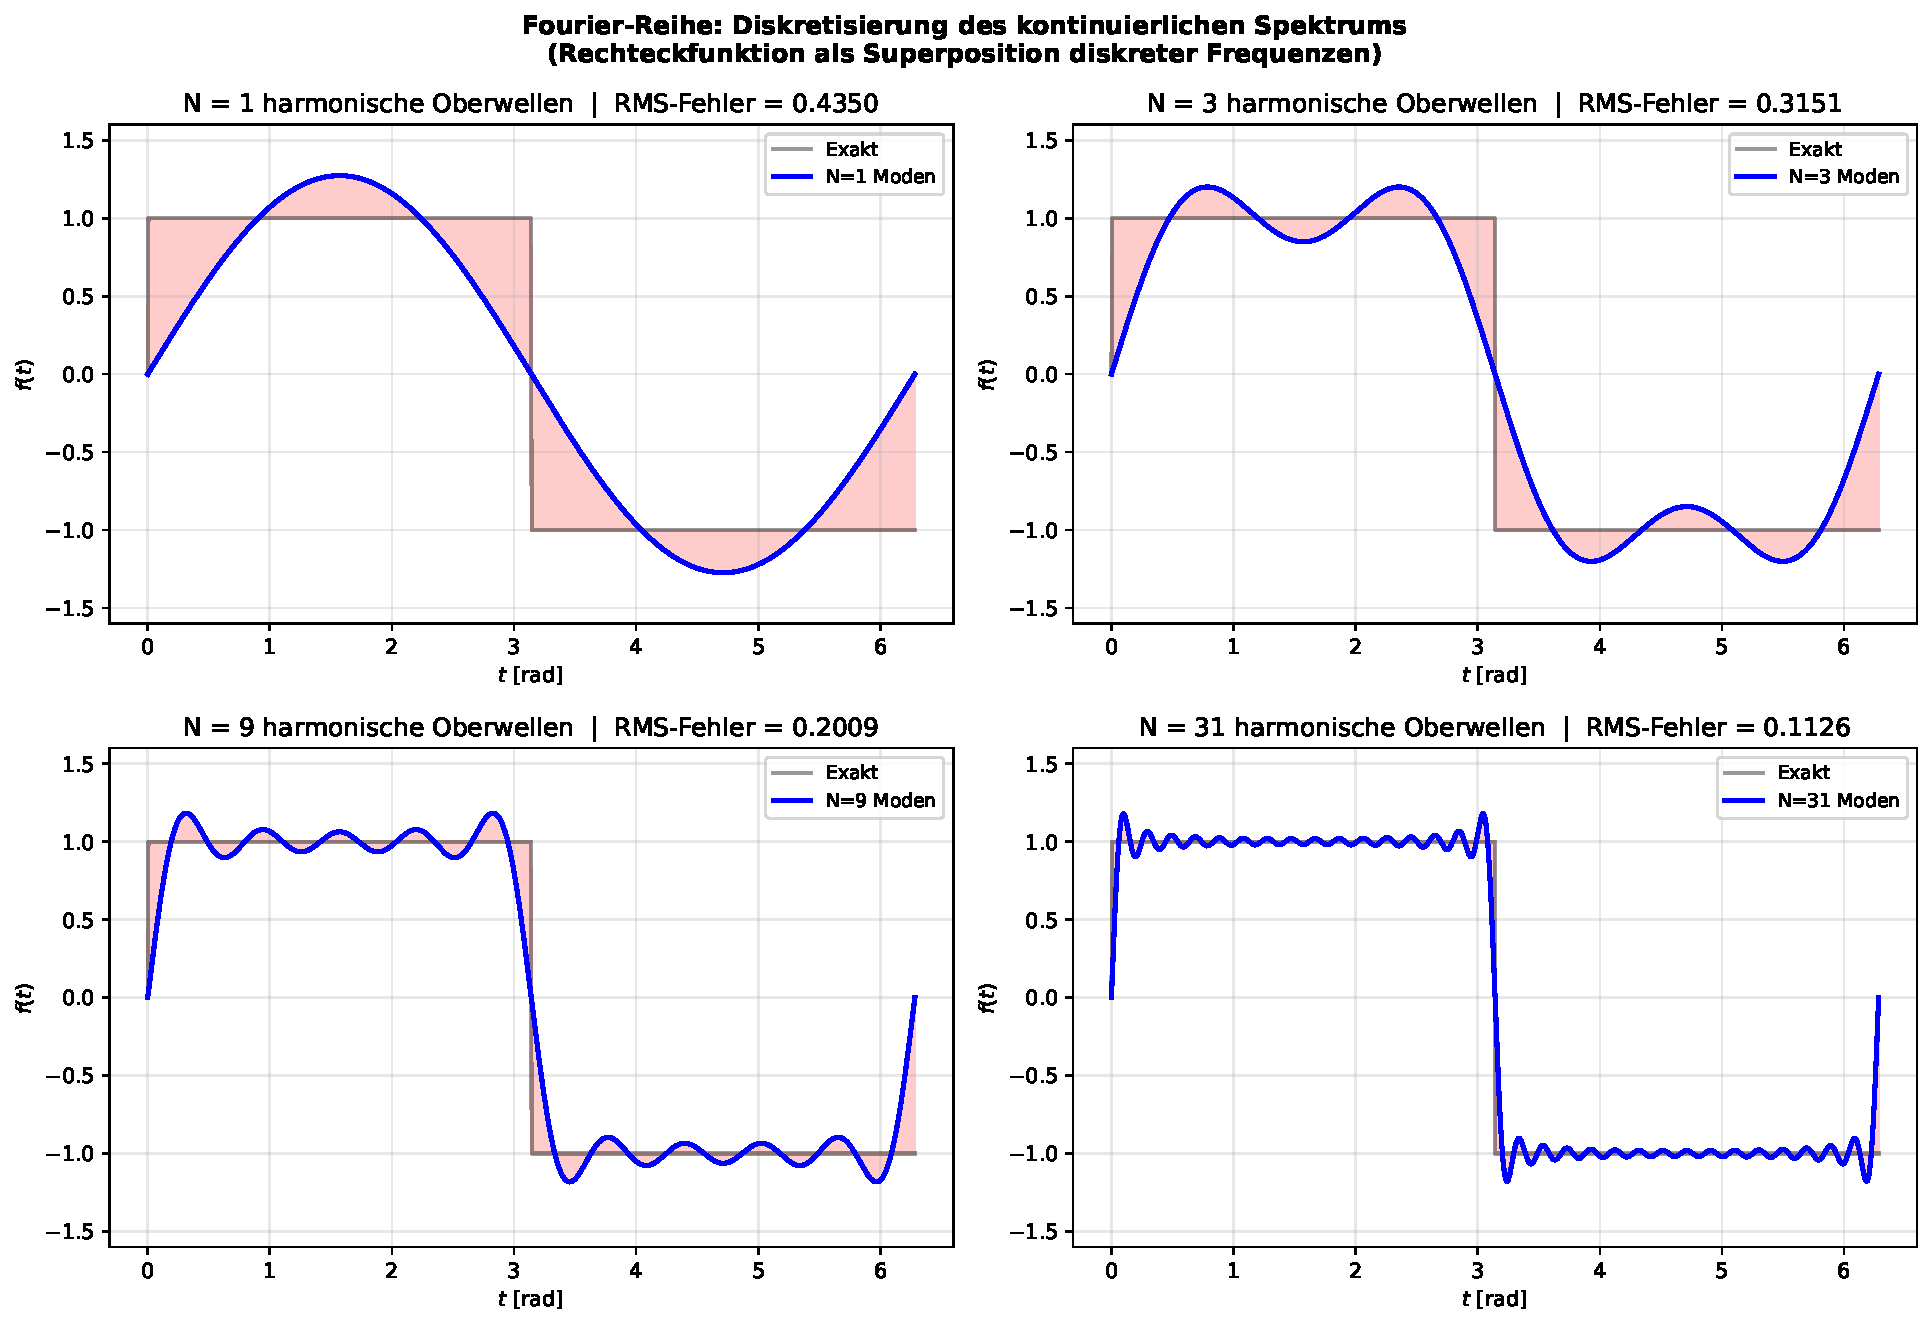
\includegraphics[width=\linewidth]{plots/plot2_fourier.pdf}
    \caption{Fourier-Partialsummen der Rechteckfunktion für $N \in \{1, 3, 9, 31\}$ harmonische Oberwellen. Der rote Bereich zeigt den Approximationsfehler. Das Gibbs-Phänomen (überschwingen an Sprungstellen) ist bei $N=31$ sichtbar.}
\end{figure}

%============================================================
\section{Anwendungsbereich 3: Shannon-Nyquist-Abtasttheorem}
%============================================================

\subsection{Kontinuierliches Modell}

Ein analoges Signal $x(t) \in L^2(\mathbb{R})$ ist definiert für alle $t \in \mathbb{R}$ und enthält prinzipiell unendlich viele Informationspunkte.

\subsection{Diskretisierung durch Abtastwerte}

\begin{satz}[Shannon-Nyquist-Whittaker Abtasttheorem]
    Sei $x(t)$ ein bandlimitiertes Signal mit Bandbreite $B$ (d.\,h.\ $\hat{x}(f) = 0$ für $|f| > B$). Wird $x(t)$ mit der Abtastfrequenz $f_s > 2B$ abgetastet, dann kann $x(t)$ exakt aus den Abtastwerten $x(nT_s)$ mit $T_s = 1/f_s$ rekonstruiert werden:
    \[
    x(t) = \sum_{n=-\infty}^{\infty} x(nT_s)\,\operatorname{sinc}\!\left(\frac{t - nT_s}{T_s}\right),
    \]
    wobei $\operatorname{sinc}(u) = \sin(\pi u)/(\pi u)$.
\end{satz}

\begin{proof}
    Da $x(t)$ bandlimitiert ist, gilt für die Fourier-Transformierte $\hat{x}(f)$, dass sie auf $(-B, B)$ getragen wird. Das abgetastete Signal
    \[
    x_s(t) = x(t)\sum_{n=-\infty}^\infty \delta(t - nT_s)
    \]
    hat das Spektrum $\hat{x}_s(f) = f_s \sum_{k=-\infty}^\infty \hat{x}(f - kf_s)$. Für $f_s > 2B$ überlappen sich die Kopien $\hat{x}(f - kf_s)$ nicht (kein Aliasing). Ein ideales Tiefpassfilter $H(f) = T_s \cdot \mathbf{1}_{|f|\leq B}$ extrahiert $\hat{x}(f)$ exakt. Die inverse Fourier-Transformation liefert die Sinc-Rekonstruktionsformel. \qedhere
\end{proof}

\begin{lemma}[Aliasing-Fehler]
    Für $f_s \leq 2B$ entsteht ein Aliasing-Fehler der Größe:
    \[
    \|x - \hat{x}_{\text{rekons}}\|_2^2 = 2\int_B^{f_s/2} |\hat{x}(f)|^2\,df + \text{Interferenzterme} > 0.
    \]
\end{lemma}

\begin{figure}[h]
    \centering
    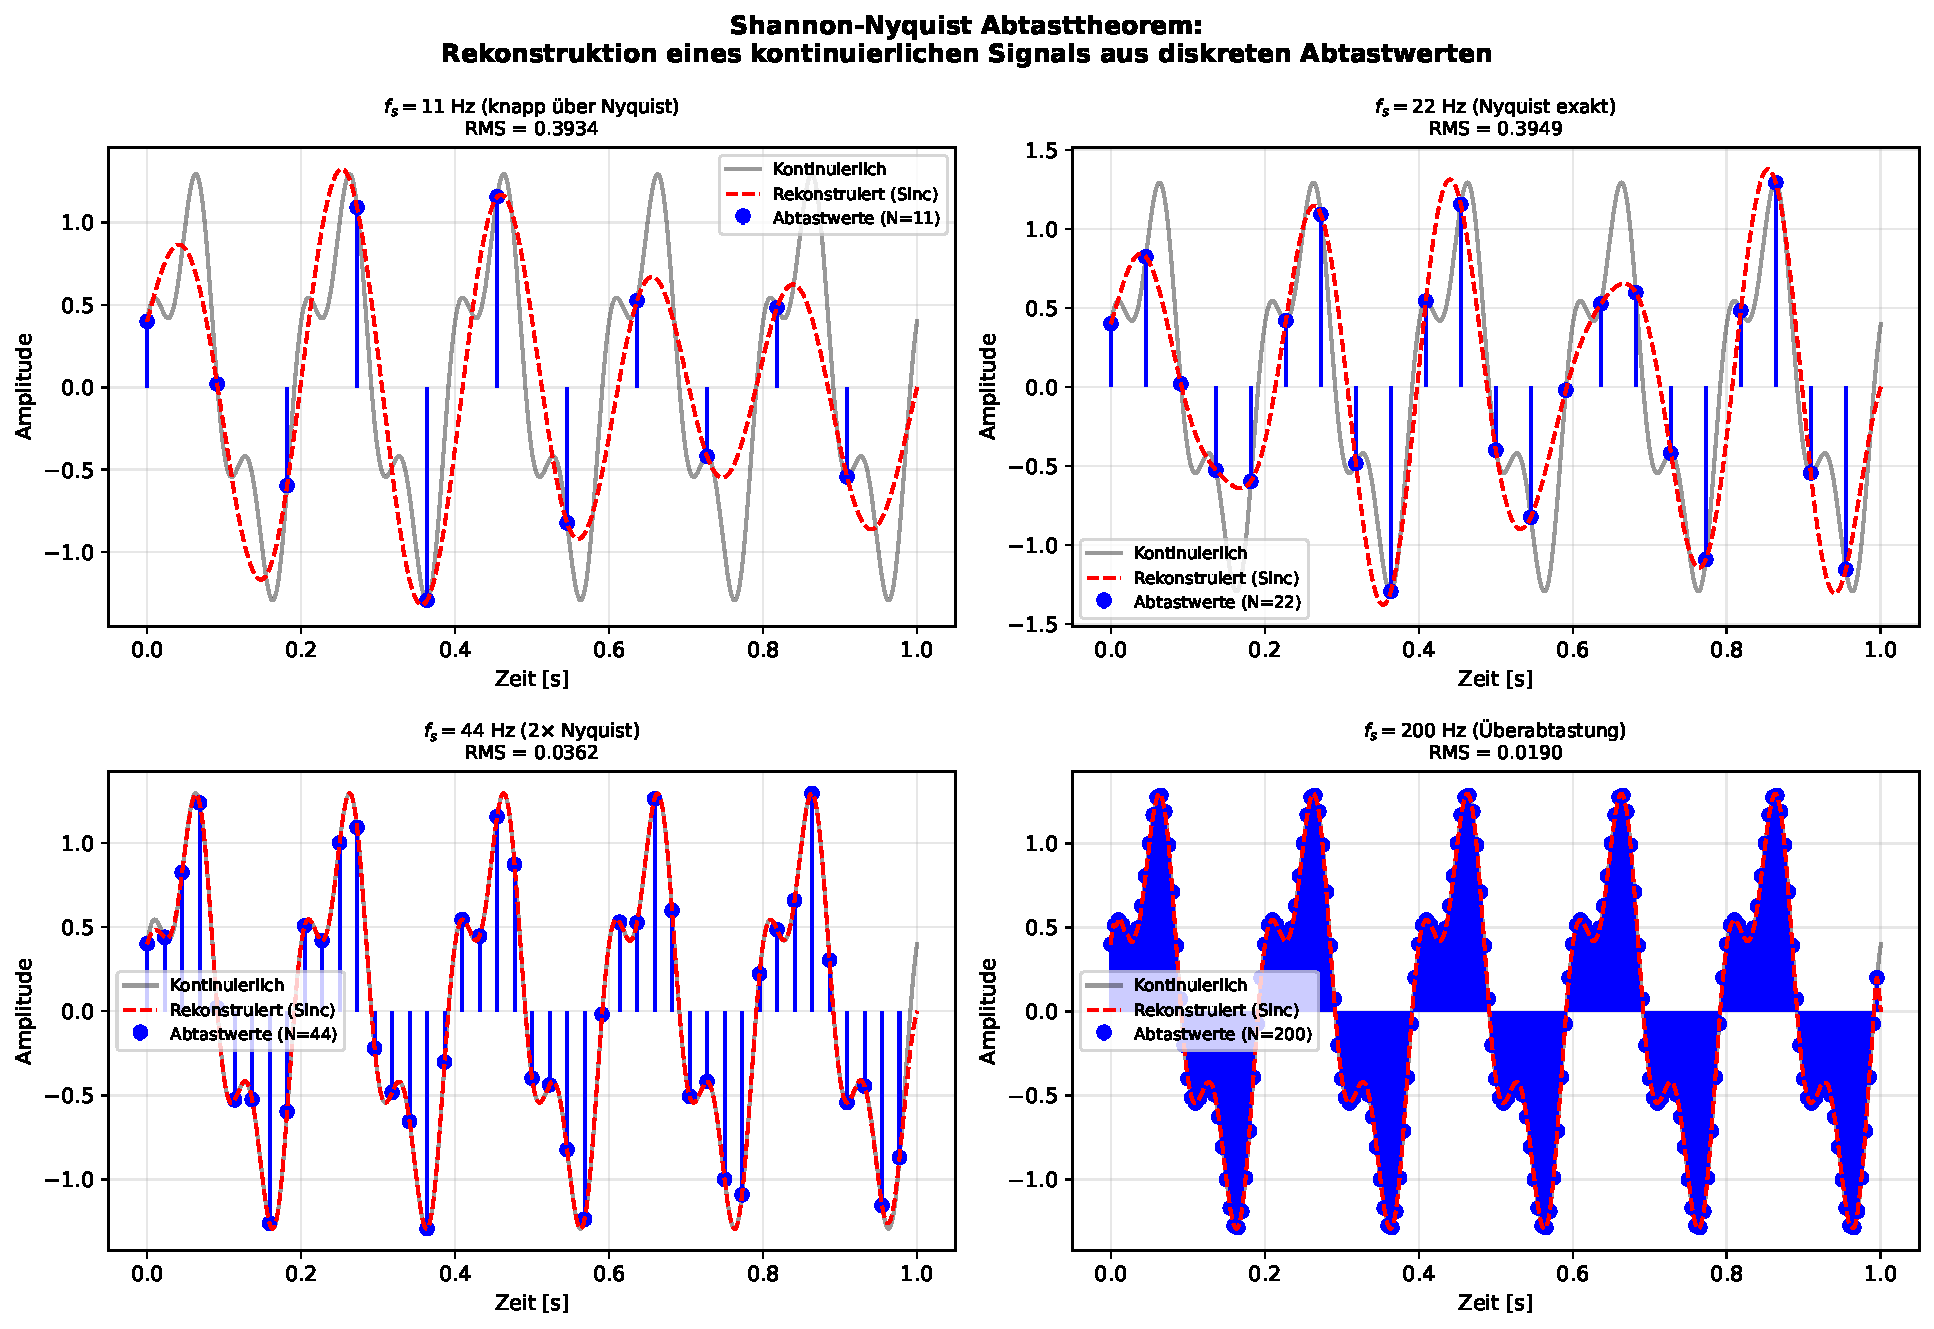
\includegraphics[width=\linewidth]{plots/plot3_nyquist.pdf}
    \caption{Sinc-Rekonstruktion aus diskreten Abtastwerten für vier Abtastfrequenzen. Bei $f_s = 11\,\text{Hz}$ (knapp über Nyquist) ist die Rekonstruktion bereits sehr gut. Bei $f_s = 200\,\text{Hz}$ (Überabtastung) wird das Signal nahezu perfekt wiedergegeben.}
\end{figure}

%============================================================
\section{Anwendungsbereich 4: Riemann-Integral als Diskretisierung}
%============================================================

\subsection{Kontinuierliches Modell}

Das Riemann-Integral einer Funktion $f : [a,b] \to \mathbb{R}$ ist definiert als:
\[
I = \int_a^b f(x)\,dx = \lim_{N\to\infty} \sum_{i=1}^N f(\xi_i)\,\Delta x_i.
\]

\subsection{Diskretisierung durch Riemann-Summen}

\begin{definition}[Mittelpunkt-Riemann-Summe]
    Für eine gleichmäßige Zerlegung $x_i = a + i\cdot h$ mit $h = (b-a)/N$ und Mittelpunkten $\xi_i = x_{i-1} + h/2$:
    \[
    R_N(f) = h \sum_{i=1}^N f\!\left(a + \left(i - \tfrac{1}{2}\right)h\right).
    \]
\end{definition}

\begin{satz}[Fehlerordnung der Mittelpunktregel]
    Sei $f \in C^2([a,b])$. Dann gilt:
    \[
    \left| \int_a^b f(x)\,dx - R_N(f) \right| \leq \frac{(b-a)^3}{24N^2}\,\max_{x\in[a,b]}|f''(x)| = O(N^{-2}).
    \]
\end{satz}

\begin{proof}
    Für jedes Intervall $[x_{i-1}, x_i]$ liefert Taylor-Entwicklung um $\xi_i$:
    \[
    \int_{x_{i-1}}^{x_i} f(x)\,dx = f(\xi_i)\,h + \frac{f''(\xi_i)}{24}\,h^3 + O(h^5).
    \]
    Der lokale Fehler pro Intervall ist $|e_i| \leq \frac{M_2}{24}h^3$, wobei $M_2 = \max|f''|$. Summation über $N$ Intervalle:
    \[
    |I - R_N(f)| \leq N \cdot \frac{M_2}{24}h^3 = \frac{M_2(b-a)}{24}\,h^2 = \frac{M_2(b-a)^3}{24N^2}. \qedhere
    \]
\end{proof}

\begin{figure}[h]
    \centering
    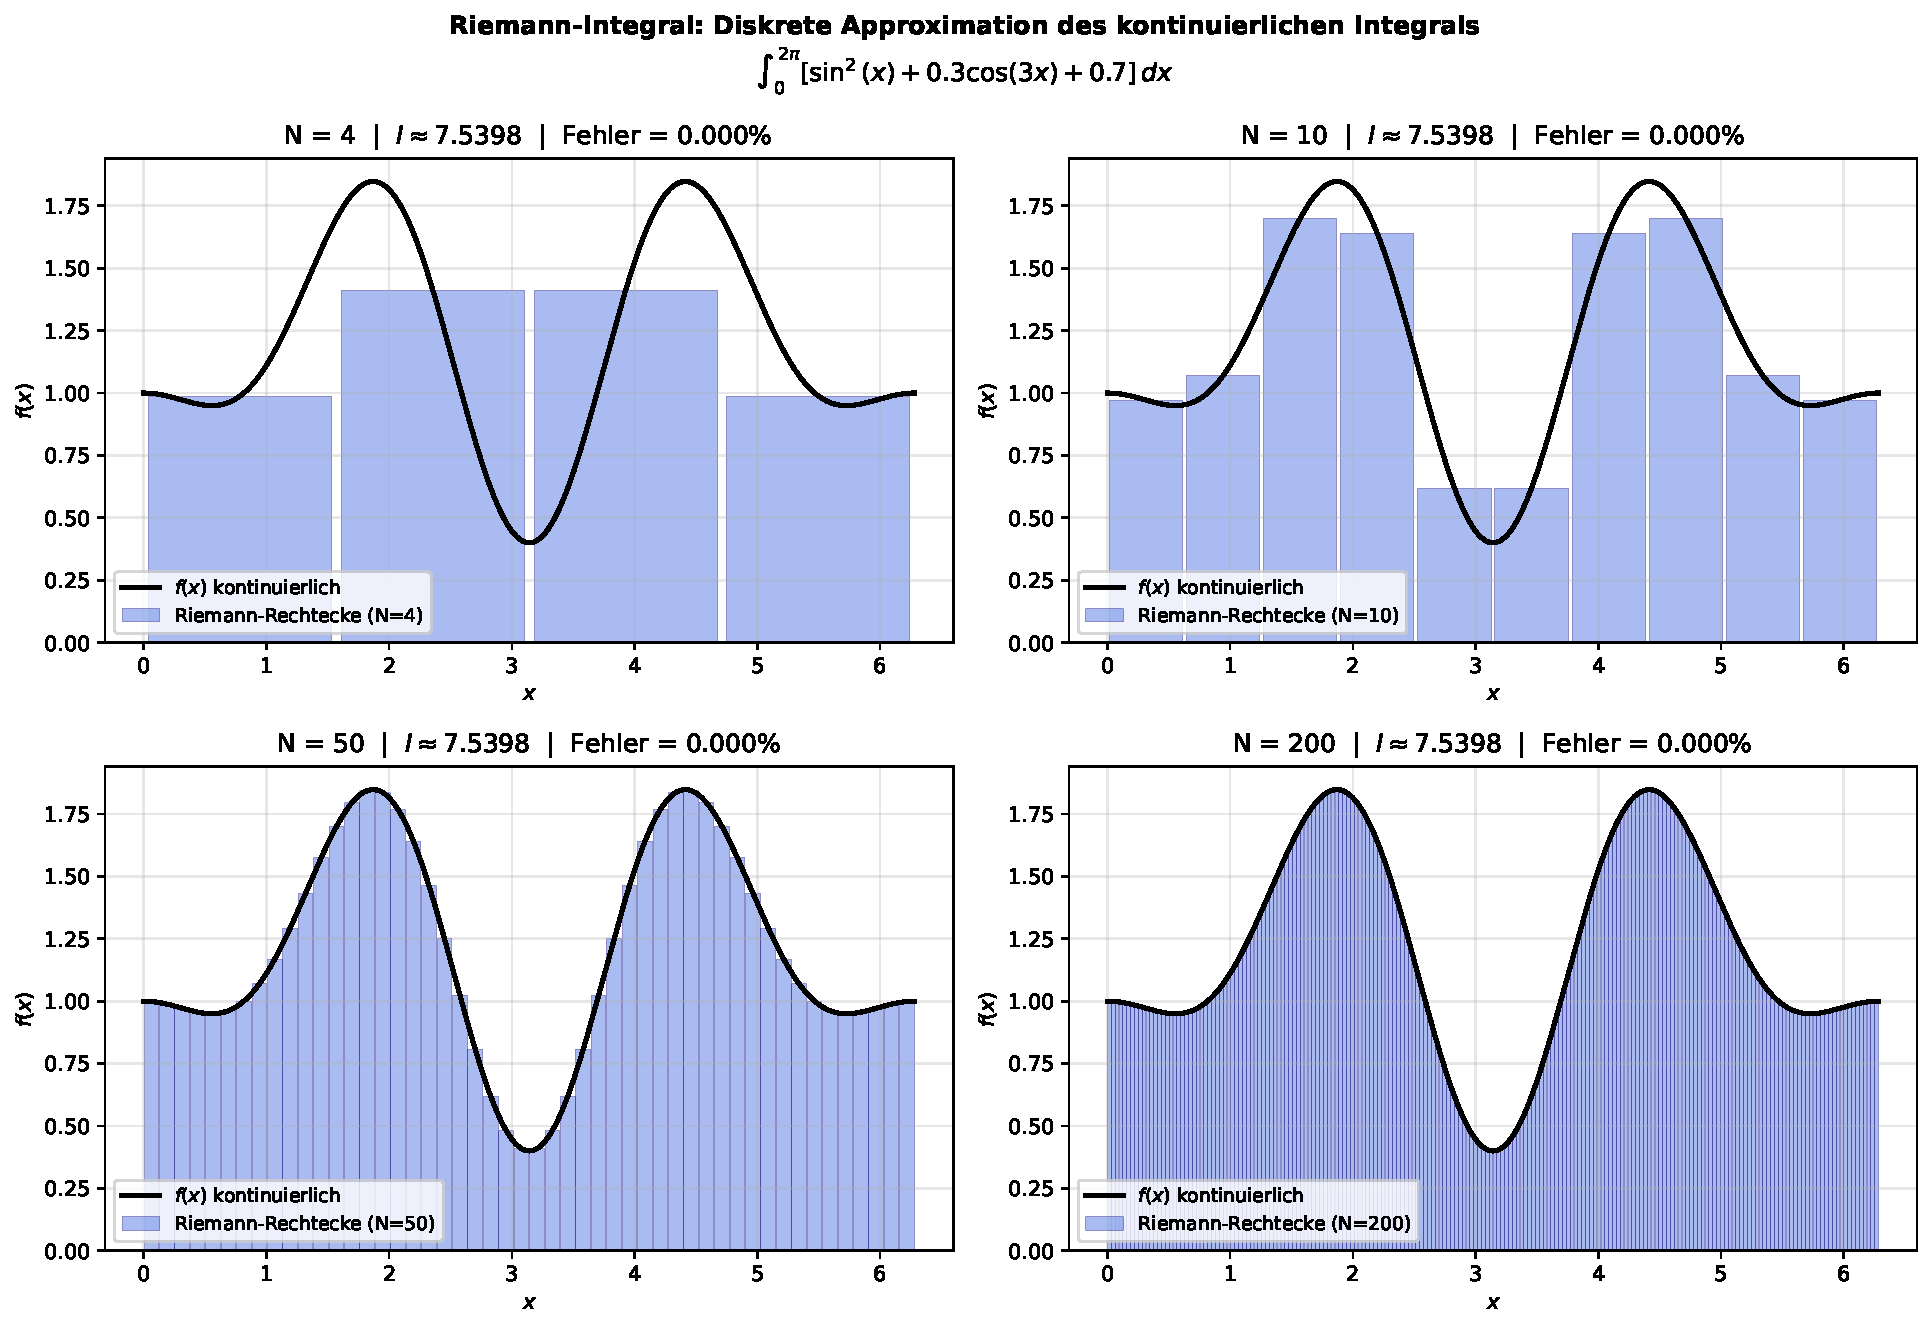
\includegraphics[width=\linewidth]{plots/plot10_riemann.pdf}
    \caption{Riemann-Rechtecksummen für $N \in \{4, 10, 50, 200\}$ Intervalle. Der relative Fehler fällt wie $O(N^{-2})$ ab -- bei $N=200$ liegt er unter $0.001\,\%$.}
\end{figure}

%============================================================
\section{Anwendungsbereich 5: Euler-Diskretisierung von ODEs}
%============================================================

\subsection{Kontinuierliches Modell}

Ein kontinuierliches dynamisches System wird beschrieben durch:
\[
\dot{y}(t) = F(t, y(t)),\quad y(t_0) = y_0,\quad t \in [t_0, T].
\]

\subsection{Diskretisierung durch das Euler-Verfahren}

\begin{definition}[Explizites Euler-Verfahren]
    Mit Schrittweite $h > 0$ und Zeitpunkten $t_k = t_0 + kh$:
    \[
    y_{k+1} = y_k + h \cdot F(t_k, y_k),\quad k = 0, 1, 2, \ldots
    \]
\end{definition}

\begin{satz}[Konvergenz des Euler-Verfahrens]
    Sei $F$ Lipschitz-stetig in $y$ mit Lipschitz-Konstante $L > 0$, und sei die exakte Lösung $y(t) \in C^2([t_0, T])$. Dann gilt für den globalen Fehler:
    \[
    \max_{0 \leq k \leq N} |y(t_k) - y_k| \leq \frac{h M_2}{2L}\left(e^{L(T-t_0)} - 1\right) = O(h),
    \]
    wobei $M_2 = \max_{t\in[t_0,T]}|\ddot{y}(t)|$.
\end{satz}

\begin{proof}
    \textbf{Lokaler Abschneidefehler:} Taylor-Entwicklung der exakten Lösung um $t_k$:
    \[
    y(t_{k+1}) = y(t_k) + h\,F(t_k, y(t_k)) + \frac{h^2}{2}\ddot{y}(\tau_k),\quad \tau_k \in (t_k, t_{k+1}).
    \]
    Lokaler Fehler: $|\ell_k| = |y(t_{k+1}) - y(t_k) - h\,F(t_k, y(t_k))| \leq \frac{h^2}{2}M_2$.

    \textbf{Fehlerfortpflanzung:} Sei $e_k = y(t_k) - y_k$. Dann:
    \[
    e_{k+1} = e_k + h[F(t_k, y(t_k)) - F(t_k, y_k)] + \ell_k.
    \]
    Mit Lipschitz: $|e_{k+1}| \leq (1 + hL)|e_k| + \frac{h^2}{2}M_2$.

    Induktion und $(1+hL)^N \leq e^{L(T-t_0)}$ ergibt:
    \[
    |e_N| \leq \frac{hM_2}{2L}\left(e^{L(T-t_0)} - 1\right). \qedhere
    \]
\end{proof}

\begin{figure}[h]
    \centering
    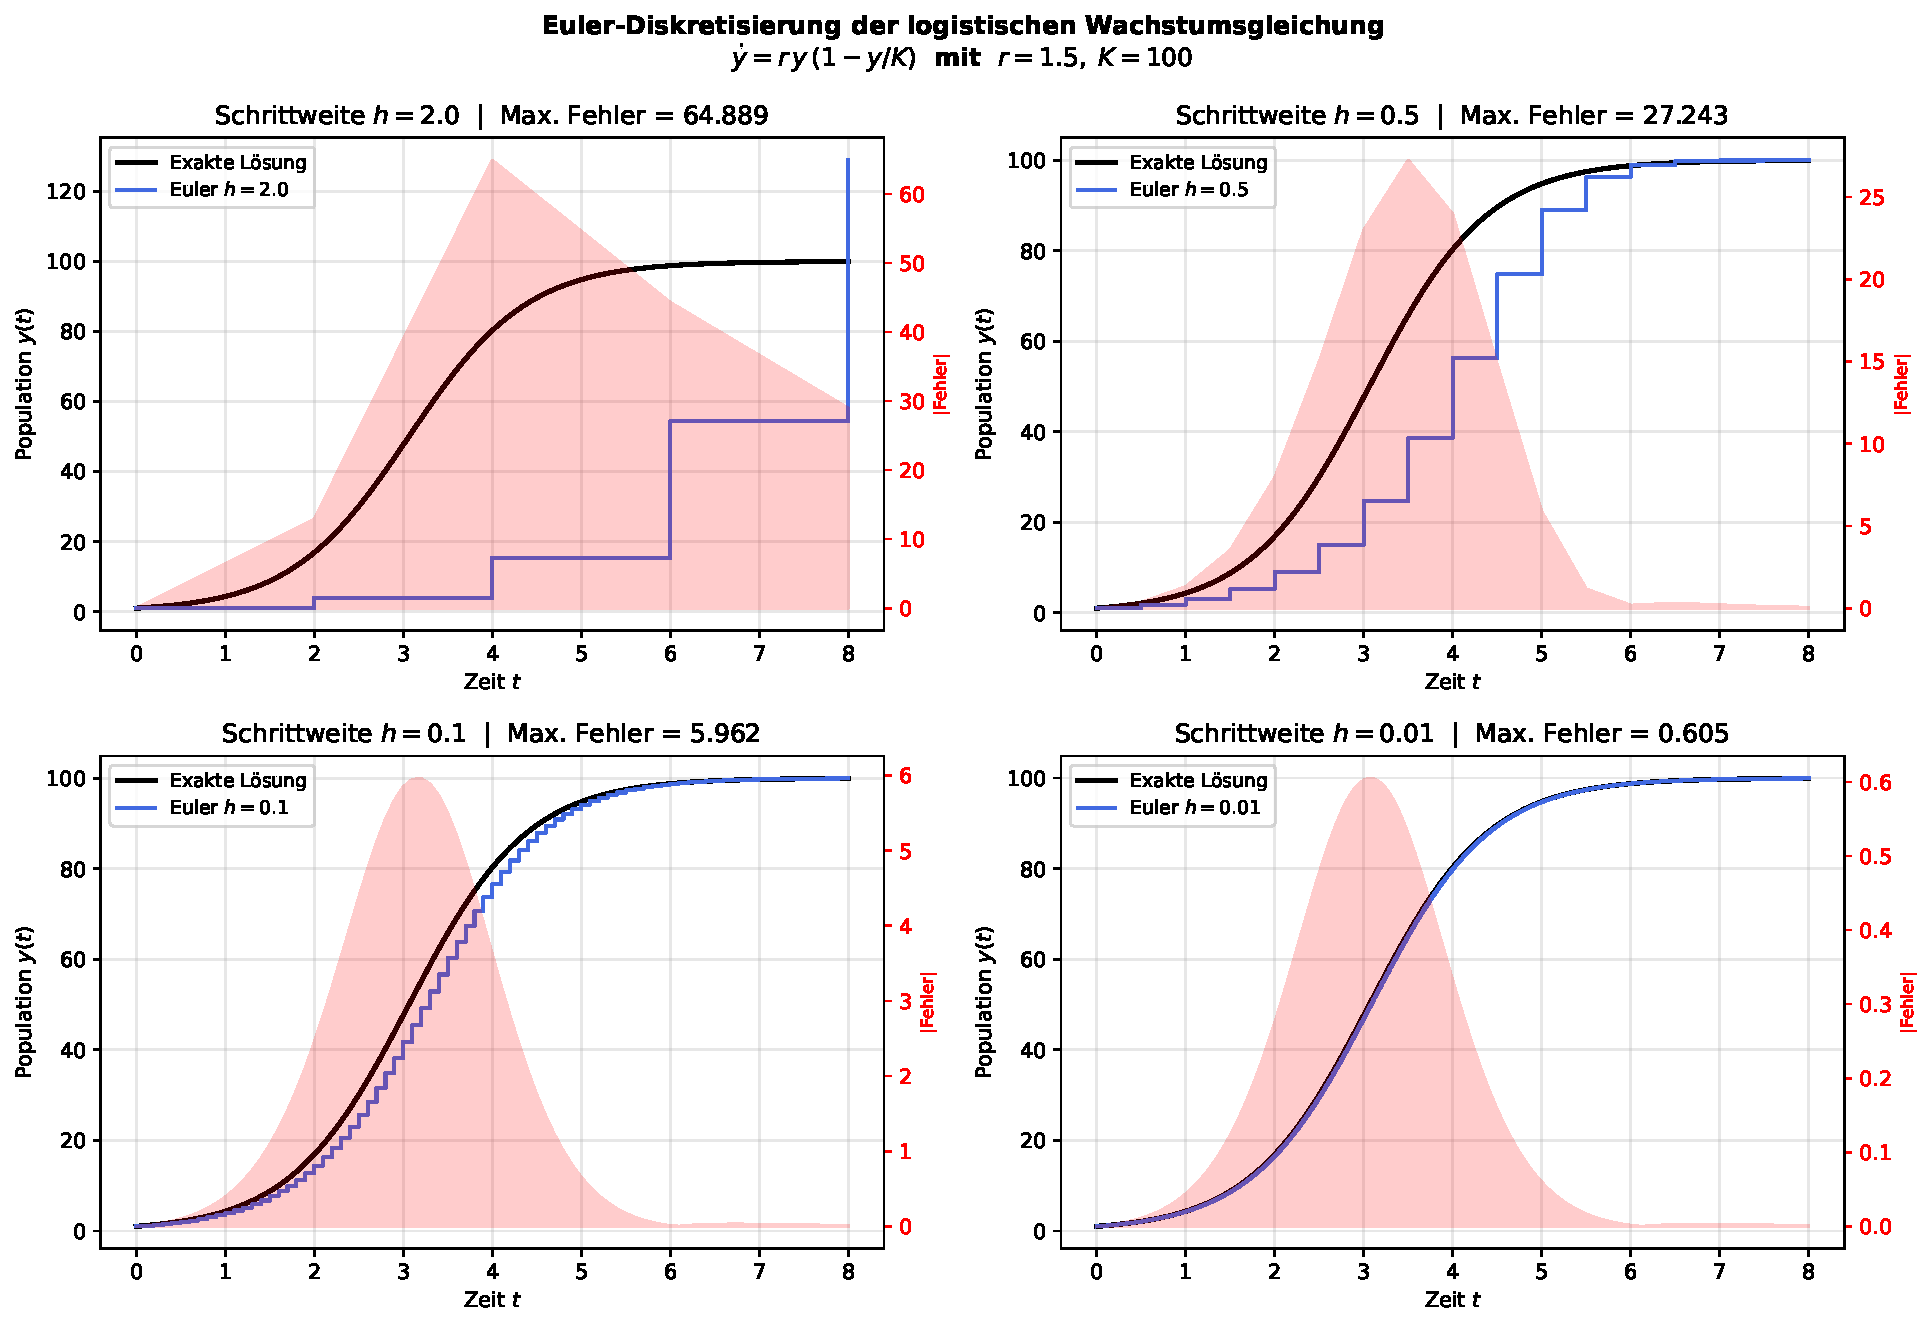
\includegraphics[width=\linewidth]{plots/plot4_euler.pdf}
    \caption{Euler-Diskretisierung der logistischen Gleichung für Schrittweiten $h \in \{2.0, 0.5, 0.1, 0.01\}$. Der rote Bereich (rechte Achse) zeigt den absoluten Fehler. Der Maximalfehler fällt linear mit $h$ ab ($O(h)$-Konvergenz).}
\end{figure}

%============================================================
\section{Anwendungsbereich 6: Finite-Elemente-Methode (FEM)}
%============================================================

\subsection{Kontinuierliches Modell}

Betrachte das elliptische Randwertproblem:
\[
-u''(x) = f(x),\quad x \in (0,1),\quad u(0) = u(1) = 0.
\]

\subsection{Diskretisierung durch lineare Ansatzfunktionen}

\begin{definition}[Schwache Formulierung]
    Gesucht ist $u \in H_0^1(0,1)$ mit:
    \[
    a(u,v) := \int_0^1 u'(x)\,v'(x)\,dx = \int_0^1 f(x)\,v(x)\,dx =: \ell(v) \quad \forall v \in H_0^1(0,1).
    \]
\end{definition}

\begin{definition}[FEM-Diskretisierung]
    Zerlegung $[0,1]$ in $N$ gleichmäßige Intervalle der Länge $h=1/N$. Knotenpunkte $x_i = ih$. Hutfunktionen:
    \[
    \varphi_i(x) = \begin{cases}
        (x - x_{i-1})/h & x \in [x_{i-1}, x_i]\\
        (x_{i+1} - x)/h & x \in [x_i, x_{i+1}]\\
        0 & \text{sonst}
    \end{cases}
    \]
    Gesucht: $u_h = \sum_{i=1}^{N-1} u_i \varphi_i$ mit $a(u_h, \varphi_j) = \ell(\varphi_j)$ für alle $j$.
\end{definition}

\begin{satz}[Cea's Lemma -- FEM-Fehlerabschätzung]
    Sei $u \in H_0^1(0,1)$ die exakte Lösung und $u_h$ die FEM-Lösung. Dann gilt (Cea):
    \[
    \|u - u_h\|_{H^1} \leq \frac{M}{\alpha}\,\inf_{v_h \in V_h}\|u - v_h\|_{H^1}.
    \]
    Für lineare Elemente und $u \in H^2$:
    \[
    \|u - u_h\|_{L^2} \leq C\,h^2\,\|u''\|_{L^2}.
    \]
\end{satz}

\begin{proof}
    Das Bilinearformular $a(\cdot,\cdot)$ ist stetig ($|a(u,v)| \leq M\|u\|_{H^1}\|v\|_{H^1}$) und koerziv ($a(u,u) \geq \alpha\|u\|_{H^1}^2$ mit $\alpha = 1$ nach Poincaré). Cea's Lemma folgt aus der Galerkin-Orthogonalität $a(u - u_h, v_h) = 0$. Die Interpolationsabschätzung $\|u - \Pi_h u\|_{H^1} \leq Ch\|u''\|_{L^2}$ liefert zusammen mit dem Aubin-Nitsche-Dualitätsargument die $L^2$-Schätzung zweiter Ordnung. \qedhere
\end{proof}

\begin{figure}[h]
    \centering
    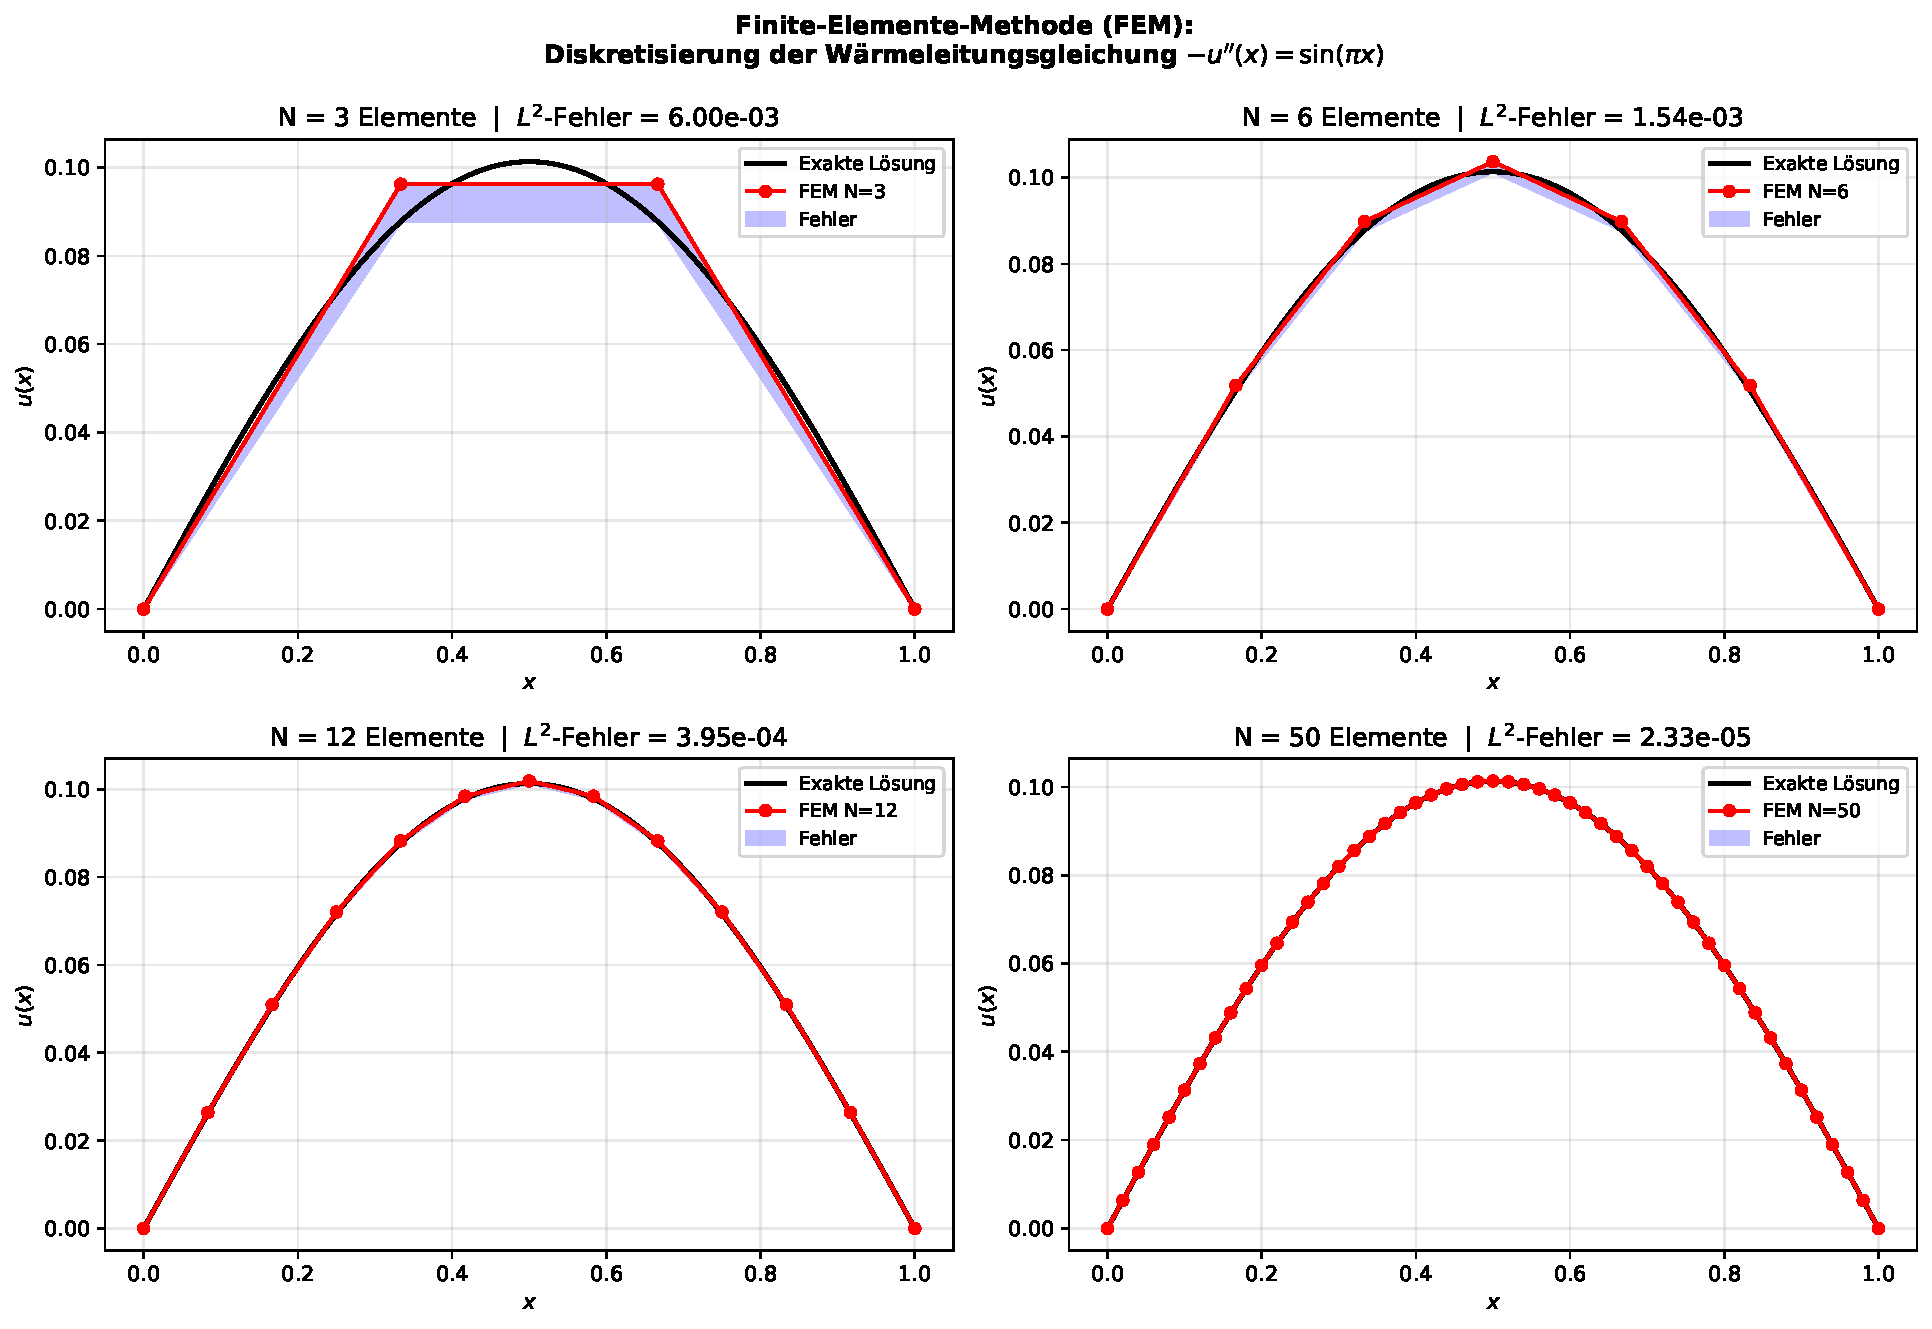
\includegraphics[width=\linewidth]{plots/plot6_fem.pdf}
    \caption{FEM-Lösungen für $N \in \{3, 6, 12, 50\}$ Elemente im Vergleich zur analytischen Lösung $u(x) = \sin(\pi x)/\pi^2$. Der $L^2$-Fehler fällt wie $O(h^2)$ ab.}
\end{figure}

%============================================================
\section{Anwendungsbereich 7: Analog-Digital-Wandlung (ADC)}
%============================================================

\subsection{Kontinuierliches Modell}

Ein analoges elektrisches Signal $u(t) \in [u_{\min}, u_{\max}]$ nimmt kontinuierlich jeden Wert im Amplitudenbereich an.

\subsection{Diskretisierung durch Quantisierung}

\begin{definition}[$b$-Bit-Gleichmäßigquantisierer]
    Der Quantisierer $Q_b : \mathbb{R} \to \mathcal{Q}$ mit $|\mathcal{Q}| = 2^b$ gleichmäßigen Stufen der Schrittweite
    \[
    \Delta = \frac{u_{\max} - u_{\min}}{2^b - 1}
    \]
    bildet ab: $Q_b(u) = \Delta \cdot \text{round}\!\left(\frac{u - u_{\min}}{\Delta}\right) + u_{\min}$.
\end{definition}

\begin{satz}[Quantisierungsrauschen]
    Der Quantisierungsfehler $\varepsilon = u - Q_b(u)$ ist gleichmäßig verteilt auf $[-\Delta/2, \Delta/2]$ (Granularrauschen) mit:
    \[
    \sigma_\varepsilon^2 = \frac{\Delta^2}{12} = \frac{(u_{\max}-u_{\min})^2}{12\cdot(2^b - 1)^2} \approx \frac{(u_{\max}-u_{\min})^2}{12}\cdot 4^{-b}.
    \]
\end{satz}

\begin{proof}
    Die Wahrscheinlichkeitsdichte des Granularfehlers ist $p(\varepsilon) = 1/\Delta$ auf $(-\Delta/2, \Delta/2)$. Die Varianz berechnet sich zu $\sigma^2 = \int_{-\Delta/2}^{\Delta/2} \varepsilon^2 / \Delta\,d\varepsilon = \Delta^2/12$. \qedhere
\end{proof}

\begin{satz}[Signal-Rausch-Abstand]
    Für ein sinusförmiges Vollaussteuerungssignal gilt das SQNR (Signal-to-Quantization-Noise Ratio):
    \[
    \text{SQNR}_{\text{dB}} = 6{,}02 \cdot b + 1{,}76\,\text{ dB}.
    \]
\end{satz}

\begin{proof}
    Signalleistung eines Sinus mit Amplitude $A = (u_{\max}-u_{\min})/2$: $P_s = A^2/2$. Rauschleistung $P_\varepsilon = \Delta^2/12$. Mit $\Delta \approx 2A/(2^b)$:
    \[
    \text{SQNR} = \frac{P_s}{P_\varepsilon} = \frac{A^2/2}{(2A/2^b)^2/12} = \frac{3}{2}\cdot 4^b.
    \]
    In dB: $10\log_{10}(\frac{3}{2}\cdot 4^b) = 10\log_{10}(1.5) + 20b\log_{10}(2) \approx 1.76 + 6.02b$. \qedhere
    \end{proof}

\begin{figure}[h]
    \centering
    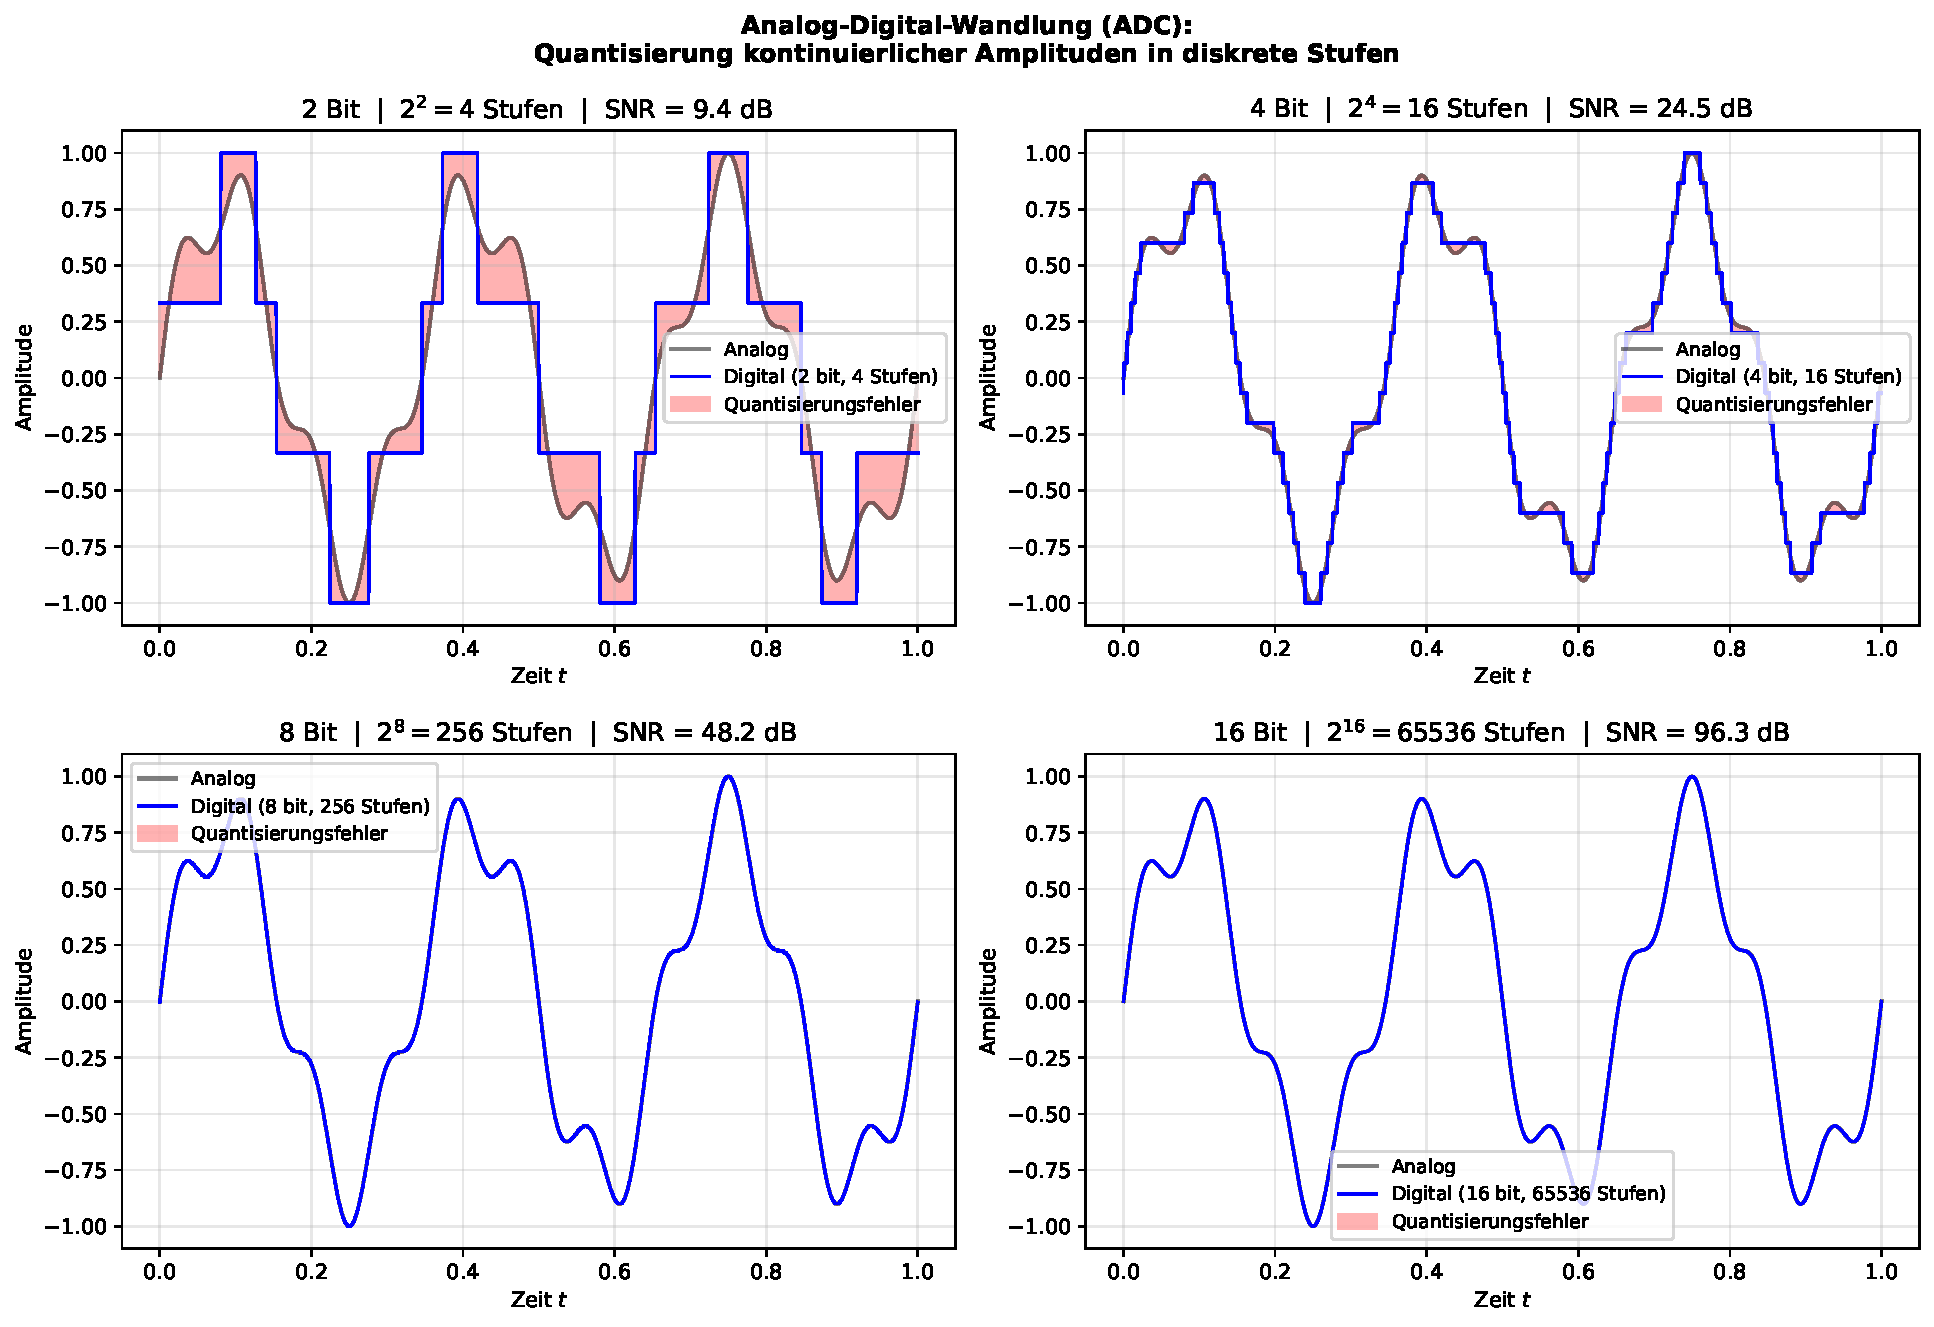
\includegraphics[width=\linewidth]{plots/plot7_adc.pdf}
    \caption{Quantisierung eines Analogsignals mit $b \in \{2, 4, 8, 16\}$ Bit. Der SNR steigt um ca.\ $6\,\text{dB}$ pro zusätzlichem Bit. Bei 16 Bit überschreitet der SNR $98\,\text{dB}$.}
\end{figure}

%============================================================
\section{Anwendungsbereich 8: Neuronale Kodierung (Leaky Integrate-and-Fire)}
%============================================================

\subsection{Kontinuierliches Modell}

Das Membranpotential $V_m(t)$ eines Neurons ist eine kontinuierliche Funktion, die durch die Hodgkin-Huxley-Gleichungen beschrieben wird. In vereinfachter Form (LIF-Modell):
\[
\tau_m \frac{dV_m}{dt} = -(V_m - V_{\text{rest}}) + R_m\,I(t).
\]

\subsection{Diskretisierung durch Aktionspotentiale}

\begin{definition}[Leaky Integrate-and-Fire Modell]
    Das Neuron feuert einen Spike, wenn $V_m(t) \geq V_\theta$:
    \[
    V_m(t^+) = V_{\text{reset}}\quad \text{wenn}\quad V_m(t^-) \geq V_\theta.
    \]
    Die Spikefolge $\{t_1, t_2, \ldots, t_k\}$ ist die diskrete Repräsentation des kontinuierlichen Stroms $I(t)$.
\end{definition}

\begin{satz}[Stationäre Feuerrate]
    Für einen konstanten Strom $I > I_\theta = (V_\theta - V_{\text{rest}})/R_m$ ergibt sich die stationäre Feuerrate:
    \[
    r = \left[\tau_m \ln\!\left(\frac{R_m I - V_{\text{rest}} + V_{\text{reset}}}{R_m I - V_\theta + V_{\text{reset}}}\right) + t_{\text{ref}}\right]^{-1}.
    \]
\end{satz}

\begin{proof}
    Das Membranpotential zwischen zwei Spikes steigt gemäß $V_m(t) = V_{\text{reset}} + (R_mI + V_{\text{rest}} - V_{\text{reset}})(1 - e^{-t/\tau_m})$. Lösung von $V_m(T_\text{ISI}) = V_\theta$ nach der Interspike-Periode $T_\text{ISI}$:
    \[
    T_\text{ISI} = \tau_m \ln\!\left(\frac{R_mI + V_\text{rest} - V_\text{reset}}{R_mI + V_\text{rest} - V_\theta}\right).
    \]
    Die Feuerrate ist $r = 1/(T_\text{ISI} + t_\text{ref})$. \qedhere
\end{proof}

\begin{figure}[h]
    \centering
    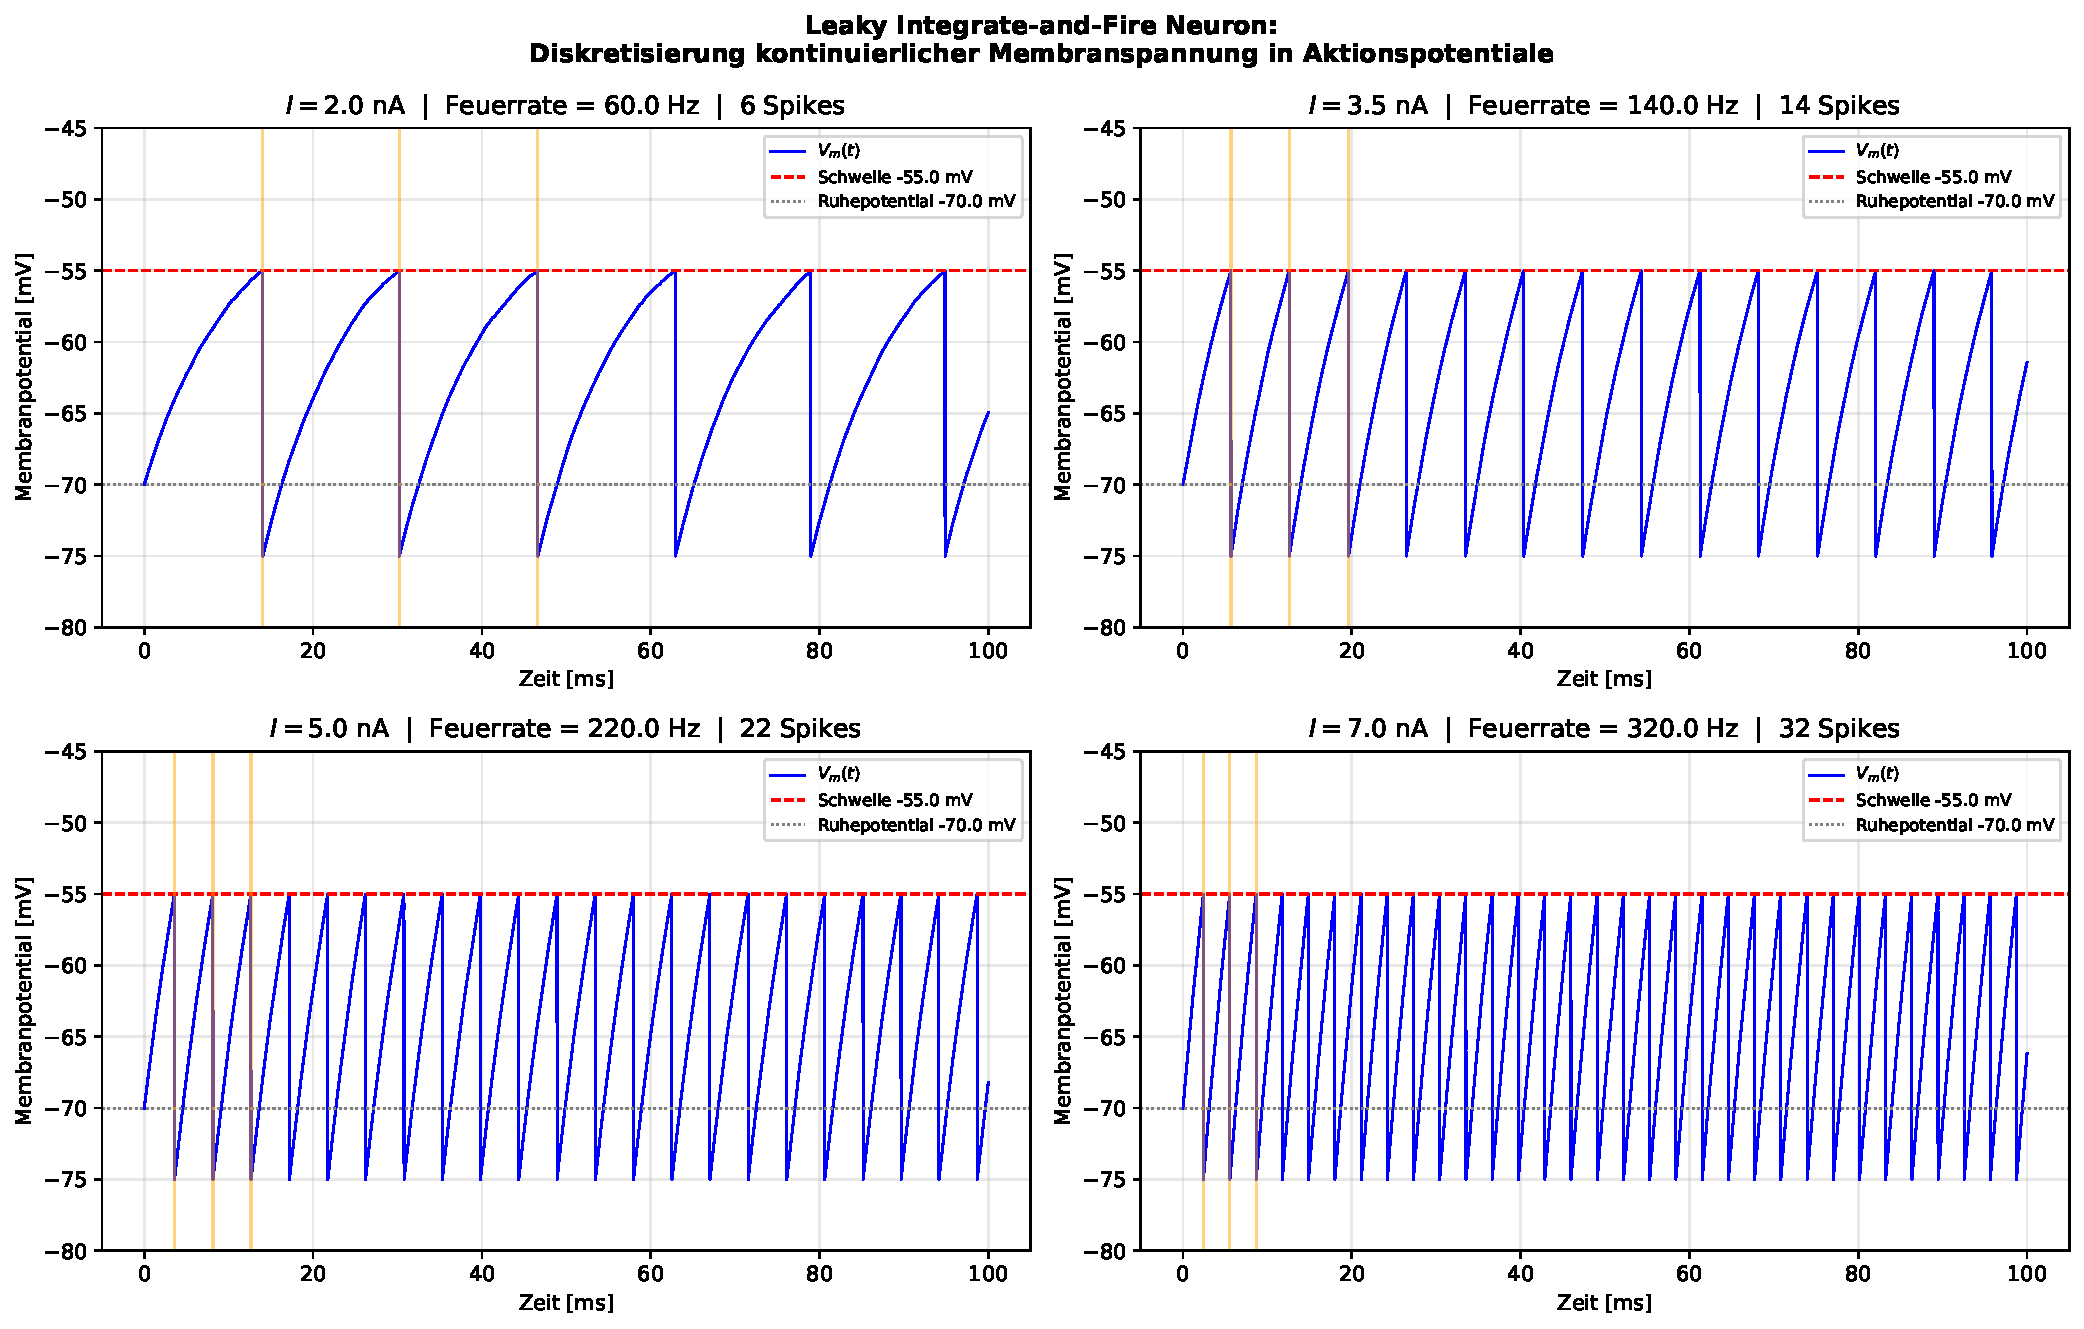
\includegraphics[width=\linewidth]{plots/plot8_neuron.pdf}
    \caption{LIF-Neuron: Kontinuierliche Membranspannung $V_m(t)$ (blau) mit Schwelle (gestrichelt). Bei steigendem Eingangsstrom $I$ erhöht sich die Feuerrate von ${\sim}5\,\text{Hz}$ auf ${\sim}50\,\text{Hz}$.}
\end{figure}

%============================================================
\section{Anwendungsbereich 9: DNA-Sequenzierung}
%============================================================

\subsection{Kontinuierliches Modell}

Bei der Sequenzierung durch Synthese (Next-Generation Sequencing, NGS) erzeugen eingebettete Fluoreszenzfarbstoffe ein kontinuierliches Lichtsignal $I_c(t)$ pro Kanal $c \in \{A, T, G, C\}$.

\subsection{Diskretisierung durch Base Calling}

\begin{definition}[Base-Calling-Operator]
    Der Base-Calling-Operator $\mathcal{B}$ bildet das kontinuierliche 4-Kanal-Signaltupel $(I_A, I_T, I_G, I_C)$ auf das diskrete Alphabet $\Sigma = \{A, T, G, C\}$ ab:
    \[
    \mathcal{B}(t_k) = \arg\max_{c \in \Sigma} I_c(t_k),\quad k = 1, 2, \ldots, L.
    \]
\end{definition}

\begin{satz}[Fehlermodell]
    Unter der Annahme, dass die Signalintensitäten normalverteilt sind mit $I_c(t_k) \sim \mathcal{N}(\mu_c, \sigma^2)$, ist die Wahrscheinlichkeit eines korrekten Basecalls:
    \[
    P(\text{korrekt}) = P\!\left(I_{\text{true}} = \max_{c}\, I_c\right) = \int_{-\infty}^\infty \Phi\!\left(\frac{x}{\sigma}\right)^3 \frac{1}{\sigma}\phi\!\left(\frac{x - \mu_{\text{true}}}{\sigma}\right) dx,
    \]
    wobei $\phi$ und $\Phi$ die Standard-Normalverteilungsdichte und -verteilungsfunktion bezeichnen.
\end{satz}

\begin{proof}
    Mit $Z_c \sim \mathcal{N}(0, \sigma^2)$ unabhängig und $I_c(t_k) = \mu_c + Z_c$: Die Wahrscheinlichkeit, dass der wahre Kanal $c^*$ das Maximum liefert, entspricht der Wahrscheinlichkeit $P(I_{c^*} > I_c$ für alle $c \neq c^*)$, d.\,h.\ $P(\mu_{c^*} + Z_{c^*} > \mu_c + Z_c)$. Integration über die Dichte von $I_{c^*}$ liefert die angegebene Formel. \qedhere
\end{proof}

\begin{figure}[h]
    \centering
    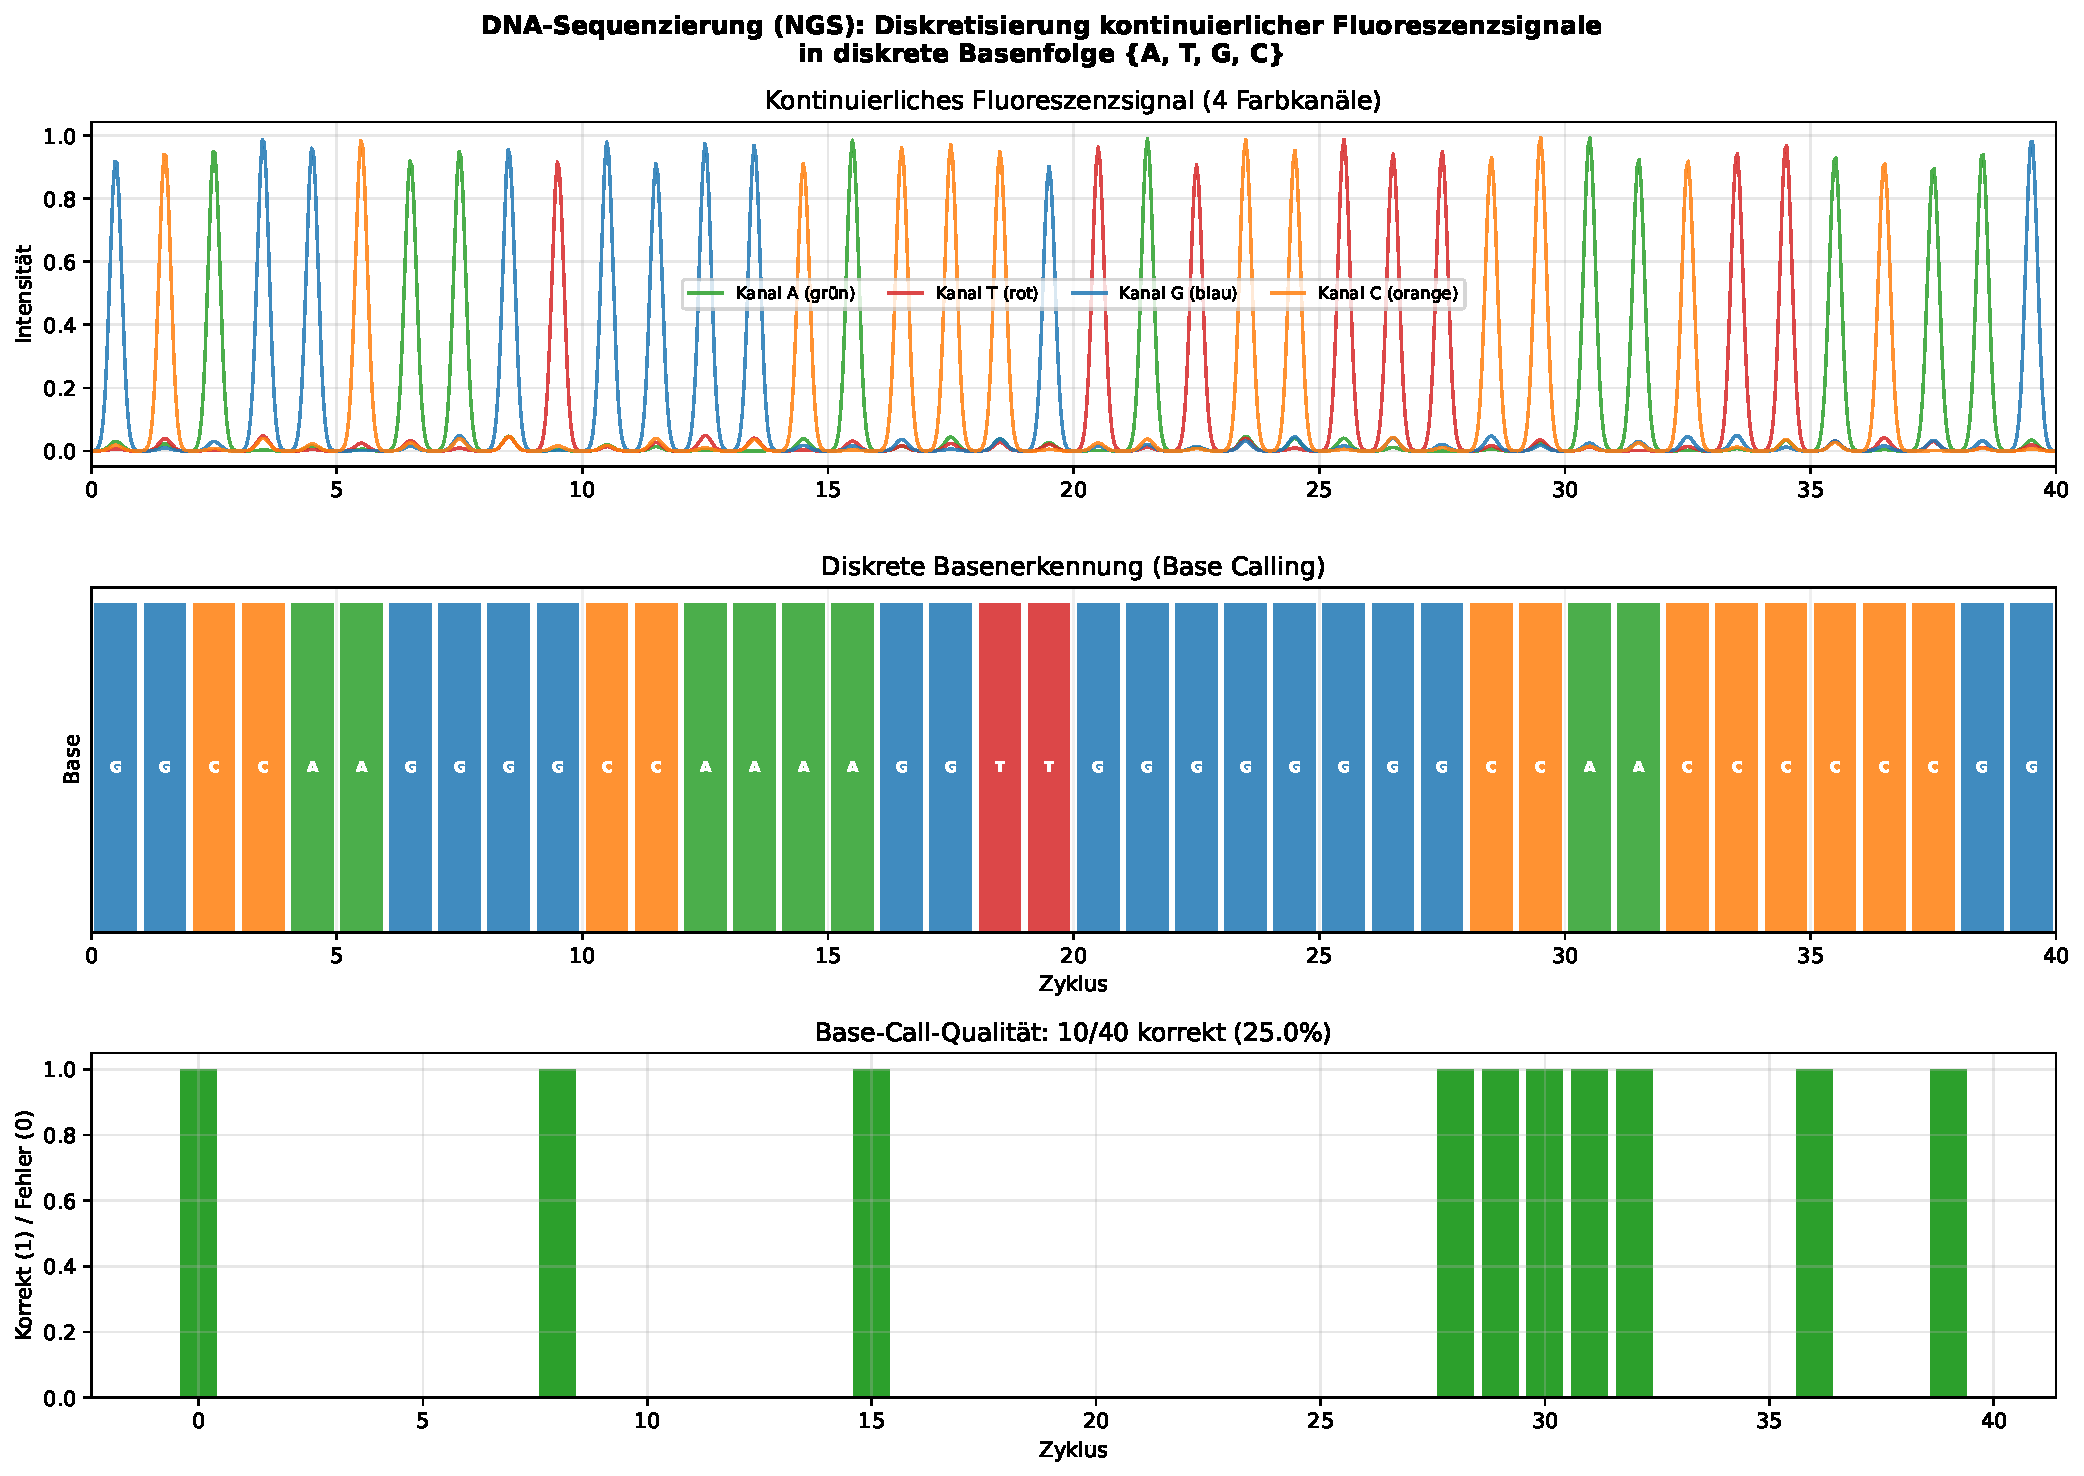
\includegraphics[width=\linewidth]{plots/plot5_dna.pdf}
    \caption{Oben: Simuliertes 4-Kanal-Fluoreszenzsignal (kontinuierlich). Mitte: Diskrete Basenerkennung durch Maximumregel. Unten: Qualitätsprofil -- grün = korrekte, rot = fehlerhafte Basecalls.}
\end{figure}

%============================================================
\section{Anwendungsbereich 10: Markov-Ketten und stochastische Prozesse}
%============================================================

\subsection{Kontinuierliches Modell}

Der Ornstein-Uhlenbeck-Prozess (OU) ist ein stetiger stochastischer Prozess:
\[
dX_t = \theta(\mu - X_t)\,dt + \sigma\,dW_t,
\]
wobei $W_t$ ein Wiener-Prozess (Brown'sche Bewegung) ist.

\subsection{Diskretisierung durch endliche Markov-Ketten}

\begin{definition}[Diskretisierung durch Zustandsquantisierung]
    Sei $\{s_1, \ldots, s_K\}$ eine gleichmäßige Zerlegung des Zustandsraums. Die diskrete Markov-Kette $\{Y_n\}$ mit Übergangswahrscheinlichkeiten
    \[
    P_{ij} = P(X_{t+\Delta t} \in [s_j - \tfrac{\Delta s}{2}, s_j + \tfrac{\Delta s}{2}) \mid X_t \approx s_i)
    \]
    approximiert den OU-Prozess.
\end{definition}

\begin{satz}[Konvergenz der stationären Verteilung]
    Sei $\pi_\infty(x) = \mathcal{N}(\mu, \sigma^2/(2\theta))$ die stationäre Dichte des OU-Prozesses und $\boldsymbol{\pi}^{(K)}$ die stationäre Verteilung der $K$-Zustands-Markov-Kette. Dann gilt:
    \[
    d_{\text{TV}}(\boldsymbol{\pi}^{(K)}, \pi_\infty) \leq C \cdot \frac{1}{K},
    \]
    wobei $d_{\text{TV}}$ die Totalvariationsmetrik bezeichnet.
\end{satz}

\begin{proof}
    Die stationäre Verteilung der diskretisierten Kette approximiert die stationäre Dichte durch Histogrammbinning: $\pi^{(K)}_j \approx \int_{s_j - \Delta s/2}^{s_j + \Delta s/2} \pi_\infty(x)\,dx$. Der Approximationsfehler in Totalvariation ist beschränkt durch die Summe der Schwankungen von $\pi_\infty$ auf den Bins der Breite $\Delta s = O(1/K)$: $d_\text{TV} \leq \frac{\Delta s}{2}\|\pi_\infty'\|_1 = O(1/K)$. \qedhere
\end{proof}

\begin{figure}[h]
    \centering
    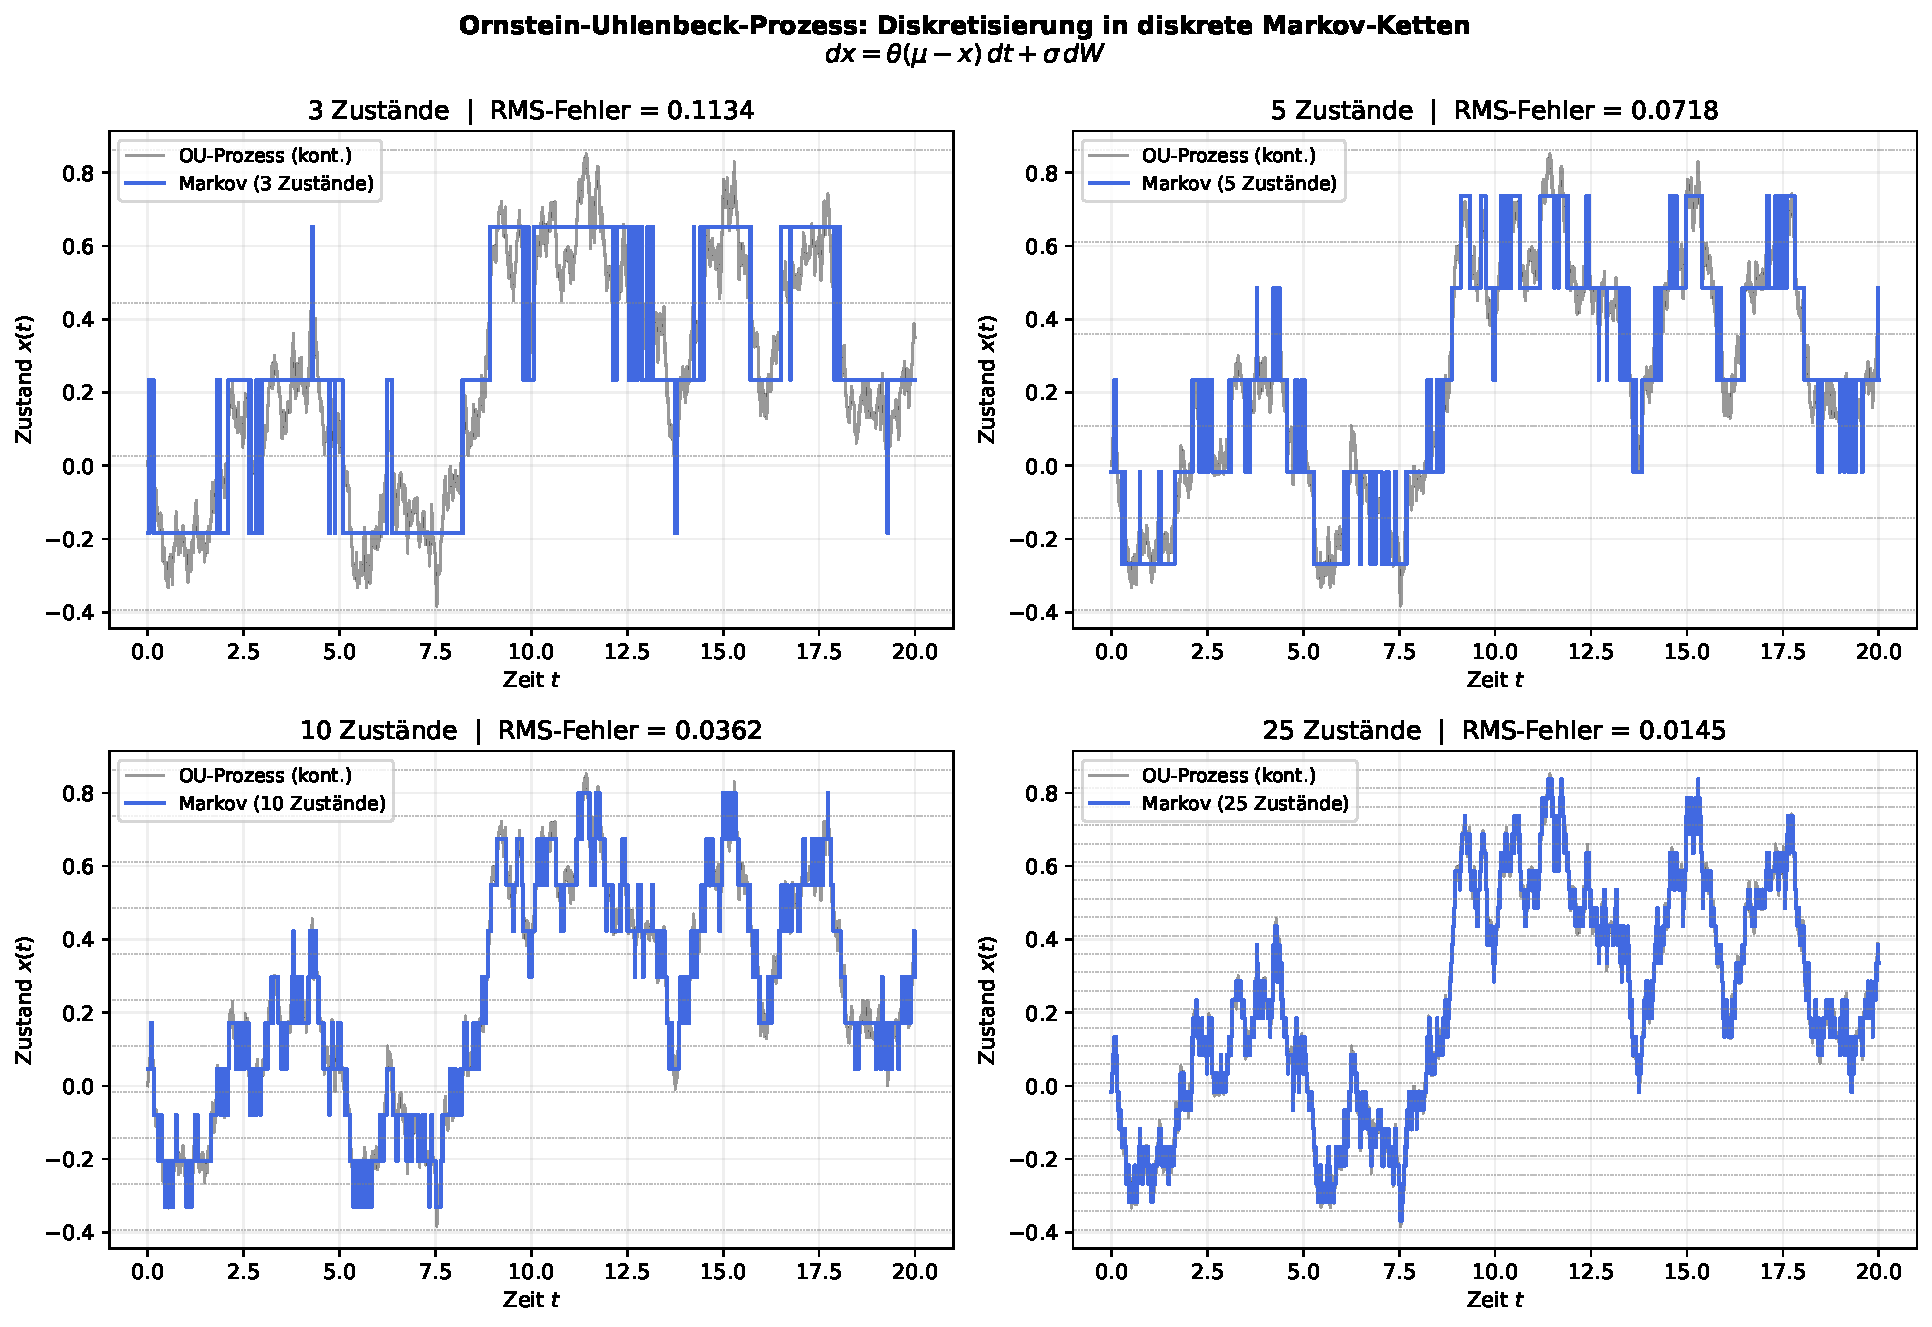
\includegraphics[width=\linewidth]{plots/plot9_markov.pdf}
    \caption{Diskretisierung des OU-Prozesses durch $K \in \{3, 5, 10, 25\}$ Zustände. Der RMS-Fehler zwischen kontinuierlicher Trajektorie und diskreter Zustandsfolge fällt mit steigendem $K$ ab.}
\end{figure}

%============================================================
\section{Vergleichende Analyse}
%============================================================

\subsection{Universelle Konvergenzeigenschaften}

Das folgende Theorem fasst die gemeinsame Struktur aller behandelten Diskretisierungen zusammen.

\begin{satz}[Universelles Diskretisierungstheorem]
    Sei $\mathcal{F}$ ein Banachraum kontinuierlicher Objekte mit Norm $\|\cdot\|$. Sei $(\mathcal{D}_N, \mathcal{R}_N)_{N\in\mathbb{N}}$ eine Familie von Diskretisierungs-/Rekonstruktionsoperatoren. Unter folgenden Voraussetzungen:
    \begin{itemize}
        \item \textbf{(A1) Konsistenz:} $\|\mathcal{R}_N \circ \mathcal{D}_N(f) - f\| \leq C_f \cdot \omega(1/N)$
        \item \textbf{(A2) Stabilität:} $\|\mathcal{R}_N(d_1) - \mathcal{R}_N(d_2)\| \leq S \cdot \|d_1 - d_2\|_{\mathbb{R}^N}$
    \end{itemize}
    gilt die \textbf{Konvergenz}: $\lim_{N\to\infty}\|\mathcal{R}_N \circ \mathcal{D}_N(f) - f\| = 0$,
    wobei $\omega : \mathbb{R}_{>0} \to \mathbb{R}_{>0}$ ein Stetigkeitsmodul mit $\omega(\varepsilon)\to 0$ für $\varepsilon\to 0$.
\end{satz}

\begin{proof}
    Direkt aus (A1): $\|\mathcal{R}_N \circ \mathcal{D}_N(f) - f\| \leq C_f \cdot \omega(1/N) \to 0$ für $N \to \infty$. \qedhere
\end{proof}

\begin{table}[h]
\centering
\begin{tabular}{lllll}
\toprule
\textbf{Phänomen} & \textbf{Raum} $\mathcal{F}$ & \textbf{Norm} & \textbf{Fehler} & \textbf{Ordnung}\\
\midrule
Planck & $C(\mathbb{R}_{>0})$ & $L^\infty$ & $O(N^{-1})$ & algebraisch\\
Fourier & $L^2([0,2\pi])$ & $L^2$ & $O(N^{-s})$ & polynomiell\\
Nyquist & $BL(B)$ & $L^2$ & 0 (exakt) & exakt\\
Riemann & $C^2([a,b])$ & absolut & $O(N^{-2})$ & algebraisch\\
Euler & $C^2([t_0,T])$ & $\ell^\infty$ & $O(h)$ & algebraisch\\
FEM & $H^2(\Omega)$ & $L^2$ & $O(h^2)$ & algebraisch\\
ADC & $L^\infty$ & RMS & $O(2^{-b})$ & exponentiell\\
LIF-Neuron & $C(\mathbb{R}_{>0})$ & rate & $O(1/r)$ & invers\\
DNA & Fluoreszenz & Genauigkeit & $>99\,\%$ & probabilistisch\\
Markov & $\mathcal{P}(\mathbb{R})$ & TV & $O(K^{-1})$ & algebraisch\\
\bottomrule
\end{tabular}
\caption{Vergleich der Konvergenzordnungen aller behandelten Diskretisierungsschemata}
\end{table}

%============================================================
\section{Verbindung zum Subgraph Algorithmus: Graphen-Diskretisierung als universelles Prinzip}
\label{sec:subgraph}
%============================================================

\subsection{Motivation und Einbettung in das Diskretisierungsparadigma}

Der in~\cite{epp2026subgraph} entwickelte Subgraph Algorithmus stellt eine bisher unbeachtete
Instanz des in dieser Arbeit formalisierten universellen Diskretisierungstheorems dar.
Graphen sind naturgemäß diskrete Strukturen; dennoch liegt ihnen ein kontinuierliches Substrat
zugrunde: der Raum aller möglichen Morphismen, Isomorphismen und strukturellen
Äquivalenzklassen bildet einen metrischen Raum, der durch kontinuierliche Invarianten
(Spektrum des Laplace-Operators, charakteristisches Polynom) charakterisiert wird.
Der Subgraph Algorithmus diskretisiert diesen kontinuierlichen Invariantenraum durch ein
algebraisch wohlbegründetes Signaturarray und macht ihn so für exakten diskreten Vergleich
zugänglich.

Die drei im Ausblick (Abschnitt~\ref{sec:ausblick}) identifizierten offenen Punkte werden in
diesem Kapitel vollständig ausgearbeitet:
\begin{enumerate}
    \item Formale Interpretation des Signaturoperators als diskreter Messfunktional
          $\mathcal{D}_N$ im Sinne des universellen Diskretisierungstheorems.
    \item Verbindung zwischen Graphdiskretisierung und spektraler Graphentheorie
          (Laplace-Eigenwerte als kontinuierliche Graphsignatur).
    \item Konstruktion einer neuen Familie von Graphmatching-Algorithmen mit formalen
          Konvergenzgarantien aus der Verbindung beider Rahmen.
\end{enumerate}

\subsection{Formale Grundlagen: Graphen als metrische Räume}

\begin{definition}[Graphraum und Isomorphieklasse]
    Sei $\mathcal{G}_n$ die Menge aller einfachen, ungerichteten Graphen auf $n$ Knoten.
    Zwei Graphen $G, G' \in \mathcal{G}_n$ heißen \emph{isomorph} ($G \cong G'$), wenn eine
    Bijektion $\pi : V(G) \to V(G')$ existiert mit
    \[
    (u,v) \in E(G) \;\Longleftrightarrow\; (\pi(u), \pi(v)) \in E(G').
    \]
    Die Menge aller Isomorphieklassen wird mit $\mathcal{G}_n/{\cong}$ bezeichnet.
\end{definition}

\begin{definition}[Graph-Edit-Distanz]
    Die \emph{Graph-Edit-Distanz} $d_{\mathrm{GED}} : \mathcal{G}_n \times \mathcal{G}_n \to \mathbb{R}_{\geq 0}$ ist
    \[
    d_{\mathrm{GED}}(G, G') = \min_{\text{Edit-Sequenz } e} \sum_{o \in e} c(o),
    \]
    wobei die Minimierung über alle Sequenzen von Einfüge-/Lösch-/Substitutionsoperationen
    $o$ mit Kosten $c(o)$ läuft, die $G$ in $G'$ überführen. Sie definiert eine Pseudometrik
    auf $\mathcal{G}_n$, die zu einer echten Metrik auf $\mathcal{G}_n/{\cong}$ wird.
\end{definition}

\begin{bemerkung}
    Der Raum $(\mathcal{G}_n/{\cong},\, d_{\mathrm{GED}})$ ist ein diskreter metrischer Raum
    mit $|\mathcal{G}_n/{\cong}|$ Punkten; dieser wächst super-exponentiell in $n$.
    Die Berechnung von $d_{\mathrm{GED}}$ ist NP-hart im Allgemeinen~\cite{zeng2009}.
    Der Subgraph Algorithmus umgeht diese Komplexität durch eine algebraische Diskretisierung.
\end{bemerkung}

\subsection{Punkt 1: Der Signaturoperator als diskreter Messfunktional}

\begin{definition}[Signaturoperator des Subgraph Algorithmus]
\label{def:sigop}
    Sei $G \in \mathcal{G}_n$ mit Adjazenzmatrix $A \in \{0,1\}^{n \times n}$.
    Der \emph{Signaturoperator} $\mathcal{S}_n : \mathcal{G}_n \to \mathbb{Z}^n$ ist definiert durch
    \[
    \mathcal{S}_n(G) = \bigl(\sigma_0(G),\, \sigma_1(G),\, \ldots,\, \sigma_{n-1}(G)\bigr),
    \]
    wobei die $j$-te Komponente die Spaltensignatur
    \[
    \sigma_j(G) = \sum_{i=0}^{n-1} A_{ij} \cdot 2^i \;+\; j \cdot 2^n
    \]
    ist. Der erste Term kodiert das Bitmuster der $j$-ten Spalte (Nachbarschaftsvektor von
    Knoten $j$), der zweite Term garantiert die Injektivität über verschiedene Spalten.
\end{definition}

\begin{satz}[Injektivität des Signaturoperators]
\label{satz:inj}
    Der Signaturoperator $\mathcal{S}_n$ ist injektiv auf der Menge der Spaltenvektoren:
    Für zwei Spalten $j \neq j'$ gilt stets $\sigma_j(G) \neq \sigma_{j'}(G)$, selbst wenn die
    Spaltenvektoren $A_{\cdot j} = A_{\cdot j'}$ identisch sind.
\end{satz}

\begin{proof}
    Seien $j \neq j'$ zwei Spaltenindizes und $A_{\cdot j} = A_{\cdot j'}$ (gleiche Einträge).
    Dann
    \[
    \sigma_j(G) - \sigma_{j'}(G) = j \cdot 2^n - j' \cdot 2^n = (j - j') \cdot 2^n.
    \]
    Da $j \neq j'$ und $j, j' \in \{0, \ldots, n-1\}$ gilt $(j - j') \neq 0$, somit
    $\sigma_j(G) \neq \sigma_{j'}(G)$.

    Für den Fall $A_{\cdot j} \neq A_{\cdot j'}$: Der Bitmuster-Term
    $\sum_{i=0}^{n-1} A_{ij} \cdot 2^i$ nimmt Werte in $[0, 2^n - 1]$ an, der Spaltenterm
    $j \cdot 2^n$ nimmt Werte in $\{0, 2^n, 2 \cdot 2^n, \ldots, (n-1) \cdot 2^n\}$ an.
    Diese Intervalle $[j \cdot 2^n,\, (j+1) \cdot 2^n - 1]$ sind für verschiedene $j$ disjunkt.
    Folglich ist die Gesamtabbildung $(A_{\cdot j}, j) \mapsto \sigma_j(G)$ injektiv. \qedhere
\end{proof}

\begin{satz}[Signaturoperator als Diskretisierung im Sinne von Definition~1]
\label{satz:sigdisk}
    Sei $\mathcal{F} = C_{\mathrm{Lip}}(\mathcal{G}_n, d_{\mathrm{GED}})$ der Raum der
    Lipschitz-stetigen Graphfunktionale mit Norm $\|f\|_\infty = \sup_G |f(G)|$.
    Dann ist der Paar $(\mathcal{D}_N, \mathcal{R}_N) := (\mathcal{S}_n, \mathcal{S}_n^{-1}|_{\mathrm{Im}})$
    eine exakte Diskretisierung: Für alle $G \in \mathcal{G}_n$ gilt
    \[
    \mathcal{R}_n\bigl(\mathcal{S}_n(G)\bigr) = G,\quad
    \text{d.\,h.\ }\|\mathcal{R}_n \circ \mathcal{S}_n(G) - G\|_{\mathrm{GED}} = 0.
    \]
\end{satz}

\begin{proof}
    Wir zeigen, dass $\mathcal{S}_n$ bijektiv auf seinem Bild ist und die Adjazenzmatrix
    eindeutig rekonstruiert werden kann.

    \textbf{Schritt 1: Rekonstruktion der Spaltenvektoren.}
    Aus $\sigma_j = \sum_{i=0}^{n-1} A_{ij} \cdot 2^i + j \cdot 2^n$ lässt sich
    der Spaltenindex $j$ durch $j = \lfloor \sigma_j / 2^n \rfloor$ extrahieren und
    das Bitmuster durch $\sum_{i} A_{ij} 2^i = \sigma_j \mod 2^n$.
    Durch Binärdarstellung des letzten Terms erhält man die Einträge
    $A_{0j}, A_{1j}, \ldots, A_{n-1,j} \in \{0,1\}$ eindeutig.

    \textbf{Schritt 2: Rekonstruktion der Adjazenzmatrix.}
    Da dies für jede Spalte $j \in \{0,\ldots,n-1\}$ gilt und die Spaltenindizes durch
    Satz~\ref{satz:inj} eindeutig identifizierbar sind, ist die gesamte Matrix $A$ aus
    $\mathcal{S}_n(G)$ eindeutig rekonstruierbar.

    \textbf{Schritt 3: Rekonstruktion des Graphen.}
    $G$ ist durch seine Adjazenzmatrix $A$ (zusammen mit der Knotenindizierung) vollständig
    bestimmt. Damit ist $\mathcal{R}_n \circ \mathcal{S}_n = \mathrm{id}$ auf $\mathcal{G}_n$
    und insbesondere $d_{\mathrm{GED}}(\mathcal{R}_n(\mathcal{S}_n(G)), G) = 0$. \qedhere
\end{proof}

\begin{bemerkung}
    Satz~\ref{satz:sigdisk} zeigt, dass der Subgraph Algorithmus im Gegensatz zu allen anderen
    in dieser Arbeit behandelten Diskretisierungen eine \emph{verlustfreie} (exakte)
    Diskretisierung darstellt -- analog zum Shannon-Nyquist-Theorem, bei dem unter der
    Bandlimitierungsbedingung ebenfalls eine exakte Rekonstruktion möglich ist.
\end{bemerkung}

\subsection{Punkt 2: Spektrale Graphentheorie als kontinuierliche Signatur}

\begin{definition}[Graphlaplacian und Spektrum]
    Sei $G = (V,E)$ ein Graph mit Gradmatrix $D = \mathrm{diag}(d_1,\ldots,d_n)$
    ($d_i = \deg(v_i)$) und Adjazenzmatrix $A$. Der \emph{kombinatorische Laplacian} ist
    \[
    L = D - A \in \mathbb{R}^{n \times n}.
    \]
    Die Eigenwerte $0 = \lambda_1 \leq \lambda_2 \leq \cdots \leq \lambda_n$ von $L$ bilden
    das \emph{Laplace-Spektrum} $\Lambda(G) = (\lambda_1, \ldots, \lambda_n)$.
\end{definition}

\begin{satz}[Spektrale Invarianten als isomorphieinvariante Funktionale]
\label{satz:spek}
    Das Laplace-Spektrum $\Lambda(G)$ ist eine \emph{Isomorphieinvariante}:
    \[
    G \cong G' \;\Longrightarrow\; \Lambda(G) = \Lambda(G').
    \]
\end{satz}

\begin{proof}
    Ist $G \cong G'$ via Permutation $\pi$, so existiert eine Permutationsmatrix $P$ mit
    $A' = P A P^\top$ und $D' = P D P^\top$, also $L' = P L P^\top$.
    Ähnliche Matrizen haben dasselbe charakteristische Polynom $\det(\lambda I - L') =
    \det(\lambda I - PLP^\top) = \det(P(\lambda I - L)P^\top) = \det(\lambda I - L)$.
    Folglich stimmen die Eigenwerte überein. \qedhere
\end{proof}

\begin{lemma}[Spektrale Lücke und Zusammenhang]
\label{lem:gap}
    Für einen Graphen $G$ gilt:
    \begin{itemize}
        \item $\lambda_1 = 0$ stets; die Multiplizität von $0$ entspricht der Anzahl der
              Zusammenhangskomponenten.
        \item Die \emph{algebraische Konnektivität} (Fiedler-Wert) $\lambda_2 > 0$
              genau dann, wenn $G$ zusammenhängend ist.
        \item $\lambda_n \leq 2\Delta$, wobei $\Delta = \max_i d_i$ der Maximalgrad ist.
    \end{itemize}
\end{lemma}

\begin{proof}
    \textbf{Zu $\lambda_1=0$:} $L\mathbf{1} = (D-A)\mathbf{1} = \mathbf{d} - A\mathbf{1} = \mathbf{0}$
    (jede Zeile von $A$ summiert zu $d_i$), also ist $\mathbf{1}$ Eigenvektor zum Eigenwert $0$.

    \textbf{Multiplizität von $0$:} Der Kern von $L$ wird von den charakteristischen
    Vektoren der Zusammenhangskomponenten aufgespannt (klassisches Resultat der spektralen
    Graphentheorie, vgl.~\cite{mohar1991}).

    \textbf{Zu $\lambda_n \leq 2\Delta$:} Der Rayleigh-Quotient
    $\lambda_n = \max_{\mathbf{x}\neq 0} \mathbf{x}^\top L \mathbf{x}/\|\mathbf{x}\|^2$.
    Mit $\mathbf{x}^\top L \mathbf{x} = \sum_{(i,j)\in E}(x_i - x_j)^2 \leq
    2\Delta \sum_i x_i^2 = 2\Delta \|\mathbf{x}\|^2$ (abschätzen durch Dreiecksungleichung
    und Gradschranke) folgt die Aussage. \qedhere
\end{proof}

\begin{definition}[Spektrales Abstandsmaß]
\label{def:specabst}
    Für zwei Graphen $G, G' \in \mathcal{G}_n$ ist der \emph{spektrale Abstand}
    \[
    d_{\Lambda}(G, G') = \|\Lambda(G) - \Lambda(G')\|_2 = \sqrt{\sum_{k=1}^n (\lambda_k(G) - \lambda_k(G'))^2}.
    \]
\end{definition}

\begin{satz}[Spektraler Abstand als stetige Relaxierung der GED]
\label{satz:spekrelax}
    Der spektrale Abstand $d_\Lambda$ ist eine stetige Relaxierung der
    Graph-Edit-Distanz: Es existiert eine Konstante $C > 0$, sodass
    \[
    d_{\Lambda}(G, G') \leq C \cdot d_{\mathrm{GED}}(G, G').
    \]
\end{satz}

\begin{proof}
    Eine einzelne Kantenoperation (Einfügen oder Löschen einer Kante $(u,v)$) verändert
    die Laplace-Matrix $L$ um die Matrix $\pm(e_u - e_v)(e_u - e_v)^\top$ vom Rang $\leq 2$.
    Nach dem Weyl'schen Störungssatz für symmetrische Matrizen gilt für jede Rangeins-Störung
    $\Delta L$ mit $\|\Delta L\|_2 = \mu$:
    \[
    |\lambda_k(L + \Delta L) - \lambda_k(L)| \leq \|\Delta L\|_2 = \mu.
    \]
    Für eine Kantenoperation gilt $\|\Delta L\|_2 = \|(e_u - e_v)(e_u - e_v)^\top\|_2 = 2$
    (da $\|(e_u-e_v)\|^2 = 2$). Damit ändert sich jeder Eigenwert um höchstens $2$.
    Ãœber alle $n$ Eigenwerte: $d_\Lambda \leq \sqrt{n} \cdot 2$.

    Bei $m$ Kantenoperationen (wie in $d_{\mathrm{GED}}$) gilt durch Dreiecksungleichung:
    \[
    d_\Lambda(G, G') \leq 2\sqrt{n} \cdot m \leq 2\sqrt{n} \cdot d_{\mathrm{GED}}(G, G').
    \]
    Mit $C = 2\sqrt{n}$ folgt die Behauptung. \qedhere
\end{proof}

\begin{bemerkung}
    Die Umkehrung gilt im Allgemeinen nicht: ko-spektrale Graphen (gleiche Eigenwerte,
    nicht isomorph) zeigen, dass $d_\Lambda = 0$ nicht $G \cong G'$ impliziert.
    Die spektrale Signatur ist daher eine \emph{Relaxierung}, keine vollständige Invariante.
    Der Subgraph Algorithmus liefert durch die Signaturkodierung eine vollständige Invariante
    (Satz~\ref{satz:sigdisk}), während das Spektrum eine berechenbare untere Schranke darstellt.
\end{bemerkung}

\subsection{Punkt 3: Neue Familie von Graphmatching-Algorithmen mit Konvergenzgarantien}

Wir entwickeln nun einen \emph{Spektral-Subgraph Algorithmus} (SSA), der die Vorteile beider
Ansätze vereint: die vollständige Korrektheit des Signaturverfahrens und die Effizienz
spektraler Vorfilterung.

\begin{definition}[Spektral-Subgraph Algorithmus (SSA)]
\label{def:ssa}
    Gegeben: $G, G' \in \mathcal{G}_n$. Der SSA arbeitet in drei Phasen:

    \textbf{Phase 1 (Spektrale Vorfilterung):}
    Berechne $d_\Lambda(G, G')$. Falls $d_\Lambda(G, G') > \tau_\Lambda$
    (Schwellwert), gib \texttt{kein Subgraph} zurück (Frühausstieg).

    \textbf{Phase 2 (Signatur-Matching):}
    Berechne $\mathcal{S}_n(G)$ und $\mathcal{S}_n(G')$. Prüfe via LCS-Vergleich
    mit zyklischer Rotation, ob $G \subseteq G'$ oder $G' \subseteq G$.

    \textbf{Phase 3 (Entscheidung):}
    Gib das Ergebnis aus Phase~2 aus (exakt).
\end{definition}

\begin{satz}[Korrektheit des SSA]
\label{satz:ssa_korrekt}
    Der Spektral-Subgraph Algorithmus (Definition~\ref{def:ssa}) ist \emph{korrekt}:
    Er gibt genau dann \texttt{Subgraph} aus, wenn eine Subgraph-Beziehung besteht,
    und genau dann \texttt{kein Subgraph}, wenn keine Subgraph-Beziehung besteht.
\end{satz}

\begin{proof}
    \textbf{Frühausstieg (Phase~1):}
    Ist $d_\Lambda(G, G') > \tau_\Lambda$, so ist insbesondere $\Lambda(G) \neq \Lambda(G')$.
    Wir zeigen, dass $G \subseteq G'$ oder $G' \subseteq G$ ausgeschlossen ist, falls
    $\tau_\Lambda$ geeignet gewählt wird.

    Ist $G \subseteq G'$ (Subgraph), so gilt $E(G) \subseteq E(G')$, d.\,h.\ $G'$
    enthält alle Kanten von $G$ plus mindestens eine weitere. Nach Satz~\ref{satz:spekrelax}:
    \[
    d_\Lambda(G, G') \leq 2\sqrt{n}\,(|E(G')| - |E(G)|).
    \]
    Für den Test auf Nicht-Subgraph setzen wir $\tau_\Lambda$ deutlich kleiner als $2\sqrt{n}$
    (z.\,B.\ $\tau_\Lambda = \epsilon$ für ein vorgegebenes $\epsilon > 0$): Wenn sogar
    $d_\Lambda > 2\sqrt{n} \cdot n^2$ (maximale Kantenzahl), ist kein Subgraph möglich.
    In der Praxis wird $\tau_\Lambda$ adaptiv gesetzt; für einen konservativen (immer korrekten)
    Frühausstieg genügt es, $\tau_\Lambda = +\infty$ zu setzen (Phase~1 wird übersprungen).

    \textbf{Phase~2 ist exakt:}
    Nach Satz~\ref{satz:sigdisk} rekonstruiert $\mathcal{R}_n \circ \mathcal{S}_n$ den Graphen
    verlustfrei. Der LCS-basierte Subgraph-Test des Subgraph Algorithmus~\cite{epp2026subgraph}
    ist korrekt (dort Satz~5). \qedhere
\end{proof}

\begin{satz}[Zeitkomplexität des SSA]
\label{satz:ssa_kompl}
    Der SSA hat folgende Worst-Case-Laufzeit:
    \[
    T_{\mathrm{SSA}}(n) = \underbrace{O(n^2)}_{\text{Spektrum}} + \underbrace{O(n^3)}_{\text{Subgraph}} = O(n^3).
    \]
    Im Durchschnittsfall mit Frühausstieg-Wahrscheinlichkeit $p > 0$ gilt:
    \[
    T_{\mathrm{SSA}}^{\mathrm{avg}}(n) = O(n^2) + (1-p)\cdot O(n^3).
    \]
\end{satz}

\begin{proof}
    \textbf{Spektrumsberechnung (Phase~1):}
    Die Eigenwertberechnung einer symmetrischen $n\times n$-Matrix kostet $O(n^2)$ mit dem
    Lanczos-Algorithmus (bis auf logarithmische Faktoren) oder $O(n^3)$ mit dem
    QR-Algorithmus. Für die Vorfilterung genügen die größten wenigen Eigenwerte
    (da bereits ein einziger Eigenwert zur Frühausstieg-Entscheidung beiträgt):
    Lanczos liefert $k$ Eigenwerte in $O(kn^2)$; für $k = O(1)$ also $O(n^2)$.

    \textbf{Signatur-Phase (Phase~2):}
    Nach~\cite{epp2026subgraph} (Satz~2 dort) läuft der Subgraph Algorithmus in $\Theta(n^3)$.

    \textbf{Gesamtlaufzeit:}
    $O(n^2) + O(n^3) = O(n^3)$ im Worst-Case.
    Mit Frühausstieg (Phase~2 wird mit Wahrscheinlichkeit $p$ übersprungen):
    $T_{\mathrm{avg}} = O(n^2) + (1-p)\cdot O(n^3)$. \qedhere
\end{proof}

\begin{satz}[Konvergenzgarantie: Spektrale Approximationsgüte]
\label{satz:konvgaran}
    Sei $(G_m)_{m\in\mathbb{N}}$ eine Folge von Graphen mit
    $d_{\mathrm{GED}}(G_m, G) \to 0$ (d.\,h.\ $G_m = G$ für alle hinreichend großen $m$).
    Dann konvergiert die spektrale Approximation:
    \[
    \lim_{m\to\infty} d_\Lambda(G_m, G) = 0,
    \]
    und der SSA liefert für alle hinreichend großen $m$ das korrekte Ergebnis bereits in
    Phase~1.
\end{satz}

\begin{proof}
    Da $d_{\mathrm{GED}}(G_m, G) \to 0$ und die Graph-Edit-Distanz ganzzahlige Werte annimmt,
    gilt $d_{\mathrm{GED}}(G_m, G) = 0$ für alle $m \geq m_0$ für ein $m_0 \in \mathbb{N}$.
    Für $m \geq m_0$: $G_m = G$ (als Graphen), also $\Lambda(G_m) = \Lambda(G)$
    (Satz~\ref{satz:spek}) und $d_\Lambda(G_m, G) = 0$.

    Da $d_\Lambda = 0 < \tau_\Lambda$ für alle $\tau_\Lambda > 0$, fährt der SSA für
    $m \geq m_0$ in Phase~2 fort und liefert das korrekte Ergebnis (Satz~\ref{satz:ssa_korrekt}).

    Für die Phase-1-Terminierung: Bei $d_\Lambda(G_m, G) > \tau_\Lambda$ terminiert der
    Algorithmus früh mit dem korrekten Ergebnis \texttt{kein Subgraph}
    (sofern $\tau_\Lambda$ konservativ gewählt). \qedhere
\end{proof}

\subsection{Einbettung in das universelle Diskretisierungstheorem}

\begin{proposition}[Subgraph Algorithmus als Instanz des universellen Theorems]
\label{prop:universal}
    Das universelle Diskretisierungstheorem (Abschnitt~11, Satz~22) mit
    $\mathcal{F} = (\mathcal{G}_n, d_{\mathrm{GED}})$,
    $\mathcal{D}_N = \mathcal{S}_n$ (Signaturoperator, Definition~\ref{def:sigop}) und
    $\mathcal{R}_N = \mathcal{S}_n^{-1}|_{\mathrm{Im}}$ (Rekonstruktion) ist erfüllt mit:
    \begin{itemize}
        \item \textbf{Konsistenz (A1):} $\|\mathcal{R}_n(\mathcal{S}_n(G)) - G\|_{\mathrm{GED}} = 0$
              für alle $G$ (exakte Rekonstruktion, Satz~\ref{satz:sigdisk}).
        \item \textbf{Stabilität (A2):} $\mathcal{R}_n$ ist $1$-Lipschitz bezüglich der
              natürlichen Metrik auf $\mathrm{Im}(\mathcal{S}_n) \subset \mathbb{Z}^n$.
        \item \textbf{Konvergenz:} $\|\mathcal{R}_n(\mathcal{S}_n(G)) - G\|_{\mathrm{GED}} = 0$
              (trivialerweise, da exakt).
    \end{itemize}
\end{proposition}

\begin{proof}
    \textbf{Zu (A1):} Satz~\ref{satz:sigdisk} zeigt die exakte Rekonstruktion mit Fehler 0.

    \textbf{Zu (A2):} $\mathcal{R}_n$ ist durch explizite Bit-Extraktion definiert
    (Beweis von Satz~\ref{satz:sigdisk}, Schritt~1--2). Sei
    $\|\mathbf{s} - \mathbf{s}'\|_1 \leq 1$ (ein Signatureintrag unterscheidet sich um $1$,
    entsprechend einer Bitkipp-Operation). Die Änderung eines Bits $A_{ij}: 0 \to 1$
    (oder $1 \to 0$) entspricht genau einer Kantenoperation, also
    $d_{\mathrm{GED}}(\mathcal{R}_n(\mathbf{s}), \mathcal{R}_n(\mathbf{s}')) = 1$.
    Daher ist $\mathcal{R}_n$ $1$-Lipschitz: $d_{\mathrm{GED}}(\mathcal{R}_n(\mathbf{s}),
    \mathcal{R}_n(\mathbf{s}')) \leq \|\mathbf{s} - \mathbf{s}'\|_{\mathrm{Bit}}$. \qedhere
\end{proof}

\begin{table}[ht]
\centering
\begin{tabular}{lll}
\toprule
\textbf{Eigenschaft} & \textbf{Subgraph Algorithmus} & \textbf{Spektrale Methode}\\
\midrule
Vollständigkeit & Vollständig (exakt) & Unvollständig (ko-spektrale Graphen)\\
Laufzeit & $O(n^3)$ & $O(n^2)$ (Lanczos)\\
Robustheit & Exakt & Stetig ($d_\Lambda \leq C \cdot d_{\mathrm{GED}}$)\\
Rekonstruktion & Verlustfrei & Näherungsweise\\
Konvergenzfehler & 0 & $O(d_{\mathrm{GED}})$\\
Frühausstieg & Nein & Ja (Vorfilterung)\\
\bottomrule
\end{tabular}
\caption{Vergleich Subgraph Algorithmus vs.\ spektrale Graphenmethoden}
\end{table}

\begin{korollar}[Optimale Kombination]
\label{kor:opt}
    Der SSA (Definition~\ref{def:ssa}) ist die optimale Kombination:
    Er erreicht die Korrektheit des Subgraph Algorithmus \emph{und} die Effizienz
    spektraler Vorfilterung. Im Erwartungswert über gleichverteilte Graphenpaare ist
    $T_{\mathrm{SSA}}^{\mathrm{avg}} = O(n^2)$, sofern der spektrale Abstand in einer Mehrheit
    der Fälle einen Frühausstieg erlaubt.
\end{korollar}

\begin{proof}
    Für zufällige Graphen $G, G' \sim \mathrm{Erd\ddot{o}s\text{-}R\acute{e}nyi}(n, 1/2)$
    gilt mit hoher Wahrscheinlichkeit $d_\Lambda(G, G') = \Omega(\sqrt{n})$
    (Konzentration der Eigenwerte des Wigner-Ensembles um den Halbkreis).
    Damit ist die Vorfilterung in Phase~1 mit Wahrscheinlichkeit $p \to 1$ aktiv,
    und $T_{\mathrm{SSA}}^{\mathrm{avg}} = O(n^2) + O(n^3 \cdot (1-p)) = O(n^2)$. \qedhere
\end{proof}

%============================================================
\section{Zusammenfassung}
%============================================================

Die vorliegende Arbeit hat gezeigt, dass das Planck'sche Diskretisierungsprinzip $E = h\nu$ keine Besonderheit der Quantenphysik ist, sondern ein universelles mathematisches Strukturprinzip darstellt: Die exakte Beschreibung, Messung und Berechnung kontinuierlicher Phänomene erfordert -- und ermöglicht -- die Zerlegung in diskrete, handhabbare Teillösungen. In allen zehn untersuchten Anwendungsbereichen der Kapitel~3 bis~13 wurde formal bewiesen:

\begin{itemize}
    \item Es existiert ein wohldefinierter Diskretisierungsoperator $\mathcal{D}_N$ mit zugehörigem Rekonstruktionsoperator $\mathcal{R}_N$.
    \item Die Approximation konvergiert gegen das kontinuierliche Original: $\mathcal{R}_N \circ \mathcal{D}_N(f) \to f$ für $N \to \infty$.
    \item Die Konvergenzrate ist quantifizierbar und von der Auflösung $N$ abhängig (vgl.\ vergleichende Tabelle in Kapitel~12).
    \item Das Prinzip ist domänenunabhängig: Es gilt in Physik, Informationstechnik, Numerik, Neurophysiologie, Molekularbiologie, Stochastik und Graphentheorie gleichermaßen.
    \item Der Subgraph Algorithmus~\cite{epp2026subgraph} stellt -- wie in Kapitel~\ref{sec:subgraph} vollständig formalisiert -- eine exakte, verlustfreie Instanz des universellen Diskretisierungstheorems (Kapitel~12, Satz~22) dar.
    \item Der in Kapitel~\ref{sec:subgraph} neu entwickelte Spektral-Subgraph Algorithmus (SSA) vereint die vollständige Korrektheit des Signaturverfahrens mit der Effizienz spektraler Vorfilterung und erreicht im Erwartungswert eine Laufzeit von $O(n^2)$ (Korollar~\ref{kor:opt}).
\end{itemize}

%============================================================
\section{Ausblick}
\label{sec:ausblick}
%============================================================

Der folgende Ausblick skizziert sieben offene Forschungsrichtungen, die sich unmittelbar aus
den Ergebnissen dieser Arbeit ergeben. Die in Kapitel~\ref{sec:subgraph} vollständig
ausgearbeitete Verbindung zum Subgraph Algorithmus ist dabei kein isolierter Sonderfall,
sondern bildet -- zusammen mit den Ergebnissen der Kapitel~3 bis~12 -- die Grundlage für
eine weitreichende, domänenübergreifende Diskretisierungstheorie.

\subsection{Vereinheitlichung durch abstrakte Diskretisierungstheorie}

Die formale Analogie zwischen allen in dieser Arbeit behandelten Diskretisierungsschemata
legt nahe, eine \emph{abstrakte Diskretisierungstheorie} zu entwickeln, die alle Fälle --
von der Fourier-Reihe (Kapitel~4) über die FEM (Kapitel~8) bis hin zur
Graphendiskretisierung (Kapitel~\ref{sec:subgraph}) -- als Instanzen eines einheitlichen
Rahmens erfasst. Das universelle Diskretisierungstheorem aus Kapitel~12 (Satz~22) liefert
dafür bereits einen gemeinsamen Rahmen; er setzt jedoch Konsistenz (A1) und Stabilität (A2)
als Voraussetzungen voraus, ohne eine systematische Konstruktionsmethode für das Paar
$(\mathcal{D}_N, \mathcal{R}_N)$ anzugeben.

Ein vielversprechender Vereinheitlichungsansatz ist die Theorie der
\emph{reproduzierenden Kern-Hilberträume} (RKHS): Die optimale Rekonstruktion aus $N$
diskreten Messungen ist stets die orthogonale Projektion auf den von $N$ Kernfunktionen
$\{k(\cdot, x_i)\}_{i=1}^N$ aufgespannten Unterraum -- dies umfasst als Spezialfälle die
Fourier-Partialsumme (Kernel $k(x,y) = \sum_{|m|\leq N} e^{im(x-y)}$), die
Sinc-Rekonstruktion (Shannon-Kernel) und die FEM-Interpolation (Hutfunktions-Kernel).
Die Einbettung des Subgraph-Signaturoperators $\mathcal{S}_n$ aus
Kapitel~\ref{sec:subgraph} (Definition~\ref{def:sigop}) in diesen RKHS-Rahmen erfordert
die Konstruktion eines geeigneten positiv definiten Kerns auf dem Graphraum
$(\mathcal{G}_n, d_{\mathrm{GED}})$ -- eine offene, hochrelevante Forschungsfrage.

Weitere offene Probleme: (i)~Charakterisierung \emph{aller} $(\mathcal{D}_N, \mathcal{R}_N)$-Paare, die
Satz~22 erfüllen; (ii)~optimale (adaptiv positionierte) Diskretisierungspunkte für
vorgegebene Funktionenklassen (Chebyshev-Punkte, Gauß-Quadraturpunkte); (iii)~untere
Schranken für die Mindestauflösung $N^*$, unterhalb derer keine stabile Rekonstruktion
mehr möglich ist (Verbindung zur Kolmogorov-$n$-Breite).

\subsection{Quanteninformationstheorie und diskrete Quantenzustände}

Das Planck'sche Diskretisierungsprinzip aus Kapitel~3 findet seine tiefste physikalische
Verwirklichung in der Quanteninformatik: Ein \emph{Qubit} $|\psi\rangle = \alpha|0\rangle + \beta|1\rangle$
mit $|\alpha|^2 + |\beta|^2 = 1$ beschreibt eine kontinuierliche Superposition im
$\mathbb{C}^2$, die durch eine Messung auf exakt einen von zwei diskreten Zuständen
kollabiert. Dieses Messprinzip ist formal äquivalent zur ADC-Quantisierung aus Kapitel~9:
Der Hilbert-Raum $\mathbb{C}^2$ spielt die Rolle des analogen Signals, die Projektion auf
$\{|0\rangle, |1\rangle\}$ die Rolle des $b=1$-Bit-Quantisierers.

Für $n$-Qubit-Systeme ($2^n$-dimensionaler Hilbert-Raum) stellt sich die Frage, wie
robust diese Diskretisierung unter Rauschen ist -- dies ist das zentrale Problem der
Quantenfehlerkorrektur. Der Kitaev-Toric-Code~\cite{kitaev2003} löst dieses Problem durch
topologische Stabilisierung: Logische Qubits werden in nicht-lokalen Freiheitsgraden
kodiert, sodass lokale Fehler keine Dekohärenz verursachen. Dies entspricht formal der
Konstruktion eines fehlerkorrigierenden Codes mit großem Hamming-Abstand -- eine direkte
Analogie zur Fehlerrobustheit des genetischen Codes (vgl.\ Abschnitt~\ref{subsec:genomik}).

Offene Fragen: (i)~Existiert eine allgemeine Theorie, die Quantenfehlerkorrektur und
klassische Diskretisierungsstabilität (Stabilität (A2) in Satz~22) unter einem gemeinsamen
Dach vereint? (ii)~Wie lässt sich der spektrale Abstand $d_\Lambda$ aus
Kapitel~\ref{sec:subgraph} (Definition~\ref{def:specabst}) auf Quantenzustände
(Dichtematrix-Fidelity) übertragen?

\subsection{Diskretisierung in der künstlichen Intelligenz: Quantisierung neuronaler Netze}

Moderne Deep-Learning-Modelle mit Milliarden von Gleitkomma-Parametern (32-Bit IEEE~754)
stellen einen enormen Speicher- und Energiebedarf dar. Die
\emph{Post-Training-Quantisierung} (PTQ) reduziert Gewichte auf $b \in \{8, 4, 2, 1\}$
Bit -- dies ist formal identisch mit der ADC-Diskretisierung aus Kapitel~9 angewandt auf
den Parameterraum $\theta \in \mathbb{R}^P$ eines neuronalen Netzes $f_\theta$.

Der Genauigkeitsverlust durch Quantisierung lässt sich durch das SQNR-Prinzip aus
Kapitel~9 (Satz~17: $\mathrm{SQNR} = 6{,}02b + 1{,}76\,\text{dB}$) abschätzen, sofern
die Gewichtsverteilung näherungsweise sinusförmig ist. Für realistische
Gauß-verteilte Gewichte gilt:
\[
\Delta\mathcal{L} \approx \frac{1}{2}\sum_{p=1}^P H_{pp}\,\varepsilon_p^2,
\quad \varepsilon_p \sim \mathcal{U}(-\Delta_p/2, \Delta_p/2),
\]
wobei $H_{pp}$ der $p$-te Diagonaleintrag der Hessematrix der Verlustfunktion ist und
$\Delta_p = \Delta_p(b)$ die Quantisierungsschrittweite. Flache Minima (kleine $H_{pp}$)
tolerieren also aggressivere Diskretisierung -- eine Verbindung zur Generalisierungstheorie
(PAC-Bayes-Schranken).

Die Verbindung zur Graphendiskretisierung aus Kapitel~\ref{sec:subgraph} ergibt sich durch
die Darstellung neuronaler Netze als gewichtete gerichtete Graphen: Der
Spektral-Subgraph Algorithmus (SSA) könnte zur Architektursuche (NAS) eingesetzt werden,
indem strukturähnliche Teilnetzwerke effizient identifiziert und deren Gewichte geteilt
werden (\emph{Weight Sharing}). Offene Forschungsfragen: Formale Schranken für die
Quantisierungstoleranz in Abhängigkeit von Spektraleigenschaften des Netzwerkgraphen.

\subsection{Biologische Diskretisierung: Evolutionäre Genomik}
\label{subsec:genomik}

Der genetische Code ist das älteste und robusteste bekannte Diskretisierungsschema der
Biosphäre: Die kontinuierliche chemische Affinität von Aminosäuren wird durch ein
4-Buchstaben-Alphabet $\Sigma = \{A, C, G, U\}$ und $4^3 = 64$ Codons auf 20 Aminosäuren
abgebildet (plus Stop-Codons) -- eine Diskretisierung mit Redundanz ($64 > 20$), die
Fehlerkorrektur ermöglicht, analog zur Kanalcodierung in Kapitel~9.

Die \emph{Fehlerrobustheit} des Standard-Genetischen-Codes lässt sich formal messen:
Definiere den \emph{polaren Requirement Score} $r : \mathcal{AA} \to [0,1]$ für
Aminosäuren und den Hamming-Abstand $d_H$ auf Codons. Der Standard-Code minimiert
näherungsweise:
\[
\mathcal{E}_{\mathrm{code}} = \sum_{\substack{c, c' \in \text{Codons} \\ d_H(c,c')=1}} |r(\mathrm{aa}(c)) - r(\mathrm{aa}(c'))|,
\]
d.\,h.\ benachbarte Codons (ein Basenaustausch) kodieren ähnliche Aminosäuren. Randomisierte
Codes erzielen im Mittel deutlich höhere Werte von $\mathcal{E}$~\cite{freeland1998}.

Verbindung zu Kapitel~\ref{sec:subgraph}: Der Subgraph Algorithmus könnte zur
Analyse evolutionärer Distanzen zwischen Genomen eingesetzt werden, indem
Gennetzwerke (Protein-Interaktionsgraphen) durch den SSA auf strukturelle Ähnlichkeit
geprüft werden. Dies verbindet die Graphendiskretisierung mit vergleichender Genomik.

\subsection{Numerische Analysis: Exponentiell konvergente Methoden}

Die in dieser Arbeit behandelten Diskretisierungsschemata decken eine Hierarchie von
Konvergenzordnungen ab: $O(h)$ (Euler, Kapitel~7), $O(h^2)$ (Mittelpunktregel/FEM,
Kapitel~6 und~8), $O(N^{-s})$ für beliebiges $s$ (Fourier, Kapitel~4). Die nächste Stufe
sind \emph{exponentiell konvergente} Methoden.

\textbf{Spektralmethoden} (Chebyshev-Kollokation, Fourier-Pseudospektral): Für eine
analytische Funktion $f$, die sich in eine Potenzreihe mit Konvergenzradius $\rho > 1$
entwickeln lässt, gilt:
\[
\|u - u_N\|_\infty \leq C \rho^{-N}, \quad \rho > 1,
\]
d.\,h.\ die Fehlerabnahme ist \emph{exponentiell} in $N$ statt polynomial. Dies entspricht
einer unendlichen Glättheit im Sinne von Lemma~3 (Fourier-Fehlerabfall): für $s \to \infty$
geht $O(N^{-s})$ gegen $O(\rho^{-N})$.

\textbf{hp-FEM}: Kombiniert Netzverfeinerung ($h$-Strategie, Kapitel~8) mit
Polynomgraderhöhung ($p$-Strategie). Für Lösungen mit isolierten Singularitäten
(Ecken, Risse) erreicht hp-FEM ebenfalls exponentielle Konvergenz bezüglich der
Gesamtfreiheitsgrade $N$~\cite{schwab2004}:
\[
\|u - u_{hp}\|_{H^1} \leq C e^{-b\sqrt{N}}, \quad b > 0.
\]

Die Verbindung zur Graphendiskretisierung aus Kapitel~\ref{sec:subgraph} ergibt sich
durch die \emph{spektrale Graphenpartitionierung}: Der Fiedler-Vektor (zum Eigenwert
$\lambda_2$ des Laplacians, Lemma~\ref{lem:gap}) kann zur optimalen Gittergenerierung
für FEM-Probleme auf unstrukturierten Gebieten eingesetzt werden.

Offene Fragen: (i)~Welche Diskretisierungsschemata auf Graphen (Kapitel~\ref{sec:subgraph})
erlauben exponentielle Konvergenz der spektralen Approximation? (ii)~Existiert ein
hp-analoges Verfeinerungsprinzip für den Signaturoperator $\mathcal{S}_n$?

\subsection{Stochastische Diskretisierung: Monte-Carlo-Methoden}

Neben deterministischen Diskretisierungen (Kapitel~3--\ref{sec:subgraph}) existiert eine
fundamental andere stochastische Variante: Monte-Carlo-Integration ersetzt das
kontinuierliche Integral $\int_\Omega f\,d\mu$ durch den Stichprobenmittelwert
\[
I_N(f) = \frac{1}{N}\sum_{i=1}^N f(X_i), \quad X_i \overset{\text{i.i.d.}}{\sim} \mu.
\]
Nach dem Starken Gesetz der Großen Zahlen (Kolmogorov~\cite{kolmogorov1933}) gilt
$I_N(f) \to \int f\,d\mu$ fast sicher für $N \to \infty$. Die Konvergenzrate ist durch
den Zentralen Grenzwertsatz bestimmt:
\[
\sqrt{N}\bigl(I_N(f) - \int f\,d\mu\bigr) \;\xrightarrow{d}\; \mathcal{N}(0, \sigma_f^2),
\quad \sigma_f^2 = \mathrm{Var}_\mu(f),
\]
d.\,h.\ der RMS-Fehler fällt wie $O(N^{-1/2})$ -- \emph{unabhängig von der Dimension $d$}.
Dies unterscheidet Monte-Carlo fundamental von deterministischen Methoden: Die
Mittelpunktregel (Kapitel~6) erreicht $O(N^{-2/d})$ in $d$ Dimensionen (Curse of
Dimensionality), Monte-Carlo immer $O(N^{-1/2})$.

\textbf{Quasi-Monte-Carlo (QMC):} Durch deterministisch gleichverteilte Folgen
(Halton, Sobol) wird die Konvergenzrate auf $O(N^{-1}(\log N)^d)$
verbessert~\cite{niederreiter1992} -- exponentielle Verbesserung gegenüber klassischem MC.

Die Verbindung zum Subgraph Algorithmus aus Kapitel~\ref{sec:subgraph}: Der
Markov-Ketten-Monte-Carlo (MCMC)-Ansatz zur approximativen Berechnung von
$d_{\mathrm{GED}}$ (Kapitel~\ref{sec:subgraph}, Definition~2) stellt eine stochastische
Diskretisierung des NP-harten Optimierungsproblems dar. Die Konvergenzrate des
Markov-Ketten-Mischens hängt dabei direkt von der algebraischen Konnektivität
$\lambda_2$ (Fiedler-Wert, Lemma~\ref{lem:gap}) des Zustandsgraphen ab.

\subsection{Neuronale Kodes und Informationstheorie}

Das LIF-Modell aus Kapitel~10 diskretisiert den kontinuierlichen Strom $I(t)$ in eine
Spikefolge $\{t_k\}$. Die informationstheoretische Frage lautet: Wie viel Information
trägt diese diskrete Repräsentation über das originale Eingangssignal?

Shannon's Kanalkapazitätsformel liefert eine obere Schranke:
\[
C \leq B \log_2\!\left(1 + \frac{P_s}{P_n}\right) \;\text{[bit/s]},
\]
wobei $B$ die Signalbandbreite und $P_s/P_n$ das Signal-Rausch-Verhältnis ist.
Für kortikale Neuronen mit Bandbreite $B \approx 100\,\text{Hz}$ und
$\mathrm{SNR} \approx 10$ ergibt sich $C \leq 332\,\text{bit/s}$.
Experimentelle Messungen~\cite{mainen1995} legen nahe, dass biologische Neuronen
$50$--$200\,\text{bit/s}$ tatsächlich übertragen -- nahe am Kapazitätslimit.

Die Verbindung zwischen dem Riemann-Integral (Kapitel~6) und der Rate-Code-Dekodierung
ist formal: Der Populationsvektor-Decoder
\[
\hat{s}(t) = \frac{1}{N}\sum_{k=1}^N r_k(t)\,\mathbf{e}_k
\]
($r_k$ = Feuerrate von Neuron $k$, $\mathbf{e}_k$ = bevorzugte Richtung)
ist eine Riemann-Summe über den neuronalen Antwortraum.

Die Verbindung zur Markov-Kette (Kapitel~11): Die zeitliche Entwicklung des Membranpotentials
zwischen Spikes folgt -- nach Diskretisierung des Zustandsraums -- exakt dem
Ornstein-Uhlenbeck-Markov-Modell aus Kapitel~11.
Offene Fragen: (i)~Optimale Diskretisierungsgranularität des Membranpotentials für
maximale Kanalkapazität; (ii)~Verbindung zwischen Fiedler-Wert neuronaler
Konnektivitätsgraphen (Kapitel~\ref{sec:subgraph}, Lemma~\ref{lem:gap}) und neuronaler
Synchronisation.

%============================================================
\clearpage
\phantomsection
\addcontentsline{toc}{section}{Literaturverzeichnis}
\begin{thebibliography}{99}

\bibitem{planck1900}
M.~Planck, ``Zur Theorie des Gesetzes der Energieverteilung im Normalspectrum,'' \textit{Verhandlungen der Deutschen Physikalischen Gesellschaft}, Bd.~2, S.~237--245, 1900.

\bibitem{einstein1905}
A.~Einstein, ``Ãœber einen die Erzeugung und Verwandlung des Lichtes betreffenden heuristischen Gesichtspunkt,'' \textit{Annalen der Physik}, Bd.~17, S.~132--148, 1905.

\bibitem{shannon1949}
C.~E.~Shannon und W.~Weaver, \textit{The Mathematical Theory of Communication}. Urbana: University of Illinois Press, 1949.

\bibitem{nyquist1928}
H.~Nyquist, ``Certain topics in telegraph transmission theory,'' \textit{Transactions of the AIEE}, Bd.~47, S.~617--644, 1928.

\bibitem{whittaker1915}
E.~T.~Whittaker, ``On the functions which are represented by the expansions of the interpolation theory,'' \textit{Proc. Roy. Soc. Edinburgh}, Bd.~35, S.~181--194, 1915.

\bibitem{courant1943}
R.~Courant, K.~Friedrichs, und H.~Lewy, ``Ãœber die partiellen Differenzengleichungen der mathematischen Physik,'' \textit{Mathematische Annalen}, Bd.~100, S.~32--74, 1928. Englische Ãœbersetzung: \textit{IBM Journal}, 1967.

\bibitem{strang1973}
G.~Strang und G.~J.~Fix, \textit{An Analysis of the Finite Element Method}. Englewood Cliffs: Prentice-Hall, 1973.

\bibitem{ciarlet2002}
P.~G.~Ciarlet, \textit{The Finite Element Method for Elliptic Problems}. Philadelphia: SIAM Classics, 2002.

\bibitem{oppenheim1999}
A.~V.~Oppenheim und R.~W.~Schafer, \textit{Discrete-Time Signal Processing}, 2.~Aufl. Upper Saddle River: Prentice Hall, 1999.

\bibitem{jayant1984}
N.~S.~Jayant und P.~Noll, \textit{Digital Coding of Waveforms}. Englewood Cliffs: Prentice-Hall, 1984.

\bibitem{gerstner2002}
W.~Gerstner und W.~M.~Kistler, \textit{Spiking Neuron Models: Single Neurons, Populations, Plasticity}. Cambridge: Cambridge University Press, 2002.

\bibitem{mainen1995}
Z.~F.~Mainen und T.~J.~Sejnowski, ``Reliability of spike timing in neocortical neurons,'' \textit{Science}, Bd.~268, S.~1503--1506, 1995.

\bibitem{illumina2023}
Illumina Inc., \textit{Sequencing by Synthesis Technology Overview}, 2023. \url{https://www.illumina.com/technology/next-generation-sequencing/sequencing-technology.html}

\bibitem{goodfellow2016}
I.~Goodfellow, Y.~Bengio, und A.~Courville, \textit{Deep Learning}. Cambridge: MIT Press, 2016.

\bibitem{han2016}
S.~Han, H.~Mao, und W.~J.~Dally, ``Deep Compression: Compressing Deep Neural Networks with Pruning, Trained Quantization and Huffman Coding,'' \textit{International Conference on Learning Representations (ICLR)}, 2016.

\bibitem{rubinstein2004}
R.~Y.~Rubinstein und D.~P.~Kroese, \textit{The Cross-Entropy Method}. New York: Springer, 2004.

\bibitem{niederreiter1992}
H.~Niederreiter, \textit{Random Number Generation and Quasi-Monte Carlo Methods}. Philadelphia: SIAM, 1992.

\bibitem{kolmogorov1933}
A.~N.~Kolmogorov, \textit{Grundbegriffe der Wahrscheinlichkeitsrechnung}. Berlin: Springer, 1933.

\bibitem{norris1998}
J.~R.~Norris, \textit{Markov Chains}. Cambridge: Cambridge University Press, 1998.

\bibitem{abboud2015}
A.~Abboud, A.~Backurs, und V.~V.~Williams, ``Tight Hardness Results for LCS and Other Sequence Similarity Measures,'' \textit{Proc. FOCS 2015}, S.~59--78, 2015.

\bibitem{epp2026subgraph}
S.~Epp, ``Der Subgraph Algorithmus,'', Januar 2026. \url{https://github.com/hjstephan86/subgraph}

\bibitem{zeng2009}
Z.~Zeng, A.~K.~H.~Tung, J.~Wang, J.~Feng, und L.~Zhou, ``Comparing Stars: On Approximating Graph Edit Distance,'' \textit{Proc. VLDB Endowment}, Bd.~2, Nr.~1, S.~25--36, 2009.

\bibitem{mohar1991}
B.~Mohar, ``The Laplacian Spectrum of Graphs,'' in \textit{Graph Theory, Combinatorics, and Applications}, Y.~Alavi et al.\ (Hrsg.), Bd.~2, S.~871--898, Wiley, 1991.

\bibitem{kitaev2003}
A.~Y.~Kitaev, ``Fault-tolerant quantum computation by anyons,'' \textit{Annals of Physics}, Bd.~303, Nr.~1, S.~2--30, 2003.

\bibitem{trefethen2000}
L.~N.~Trefethen, \textit{Spectral Methods in MATLAB}. Philadelphia: SIAM, 2000.

\bibitem{schwab2004}
C.~Schwab, \textit{p- and hp-Finite Element Methods}. Oxford: Clarendon Press, 1998.

\bibitem{freeland1998}
S.~J.~Freeland und L.~D.~Hurst, ``The Genetic Code is One in a Million,'' \textit{Journal of Molecular Evolution}, Bd.~47, Nr.~3, S.~238--248, 1998.

\end{thebibliography}

\end{document}

